\documentclass[12pt]{report}
\usepackage{float}
\usepackage{graphicx}
\usepackage{wrapfig}
\usepackage{pythonhighlight}

\usepackage{listings}
\usepackage{color}
\definecolor{lightgray}{rgb}{.9,.9,.9}
\definecolor{darkgray}{rgb}{.4,.4,.4}
\definecolor{purple}{rgb}{0.65, 0.12, 0.82}
%\graphicspath{ {/Users/andreaolivari/Dropbox/tesi/latex/img/} }

\lstdefinelanguage{javascript}{
  keywords={typeof, new, true, false, catch, function, return, null, catch, switch, var, if, in, while, do, else, case, break},
  keywordstyle=\color{blue}\bfseries,
  ndkeywords={class, export, boolean, throw, implements, import, this},
  ndkeywordstyle=\color{darkgray}\bfseries,
  identifierstyle=\color{black},
  sensitive=false,
  comment=[l]{//},
  morecomment=[s]{/*}{*/},
  commentstyle=\color{purple}\ttfamily,
  stringstyle=\color{red}\ttfamily,
  morestring=[b]',
  morestring=[b]"
}

\lstset{
   language=javascript,
   backgroundcolor=\color{white},
   extendedchars=true,
   basicstyle=\footnotesize\ttfamily,
   showstringspaces=false,
   showspaces=false,
   numbers=left,
   numberstyle=\footnotesize,
   numbersep=9pt,
   tabsize=2,
   breaklines=true,
   showtabs=false,
   captionpos=b
}


\title{\textbf{Security analysis of protocols used in IoT solutions}}
\author{Andrea Olivari}
\date{\today}

\begin{document}

\maketitle
\tableofcontents{}

\part{MQTT}

\chapter{Protocol Overview}

\section{Introduction}
\bigskip
\textsc{MQTT} is a simple, open and light-weight standarized messaging transport protocol, based on top of TCP/IP, invented in 1999 with the following goals:

%{\addtolength{\leftskip}{5mm}
%indent
%}

\begin{itemize}
\setlength{\itemindent}{+4mm}
  \item[$\bullet$] minimal battery loss
  \item[$\bullet$] minimal bandwidth
  \item[$\bullet$] be easy simple to implement
  \item[$\bullet$] providing a good quality delivery service
\end{itemize}\
All these aspects make this protocol particularly suitable for very constrained devices, which are often used in IoT services.\\\\
Nowadays MQTT is used in many different fields of applications:

 \begin{itemize}
 \setlength{\itemindent}{+4mm}
  \item[$\bullet$] Sensors communications \textit{(light, temperature, humidity, magnetic fields, pressure, intrusion detectors, etc})
  \item[$\bullet$] Health monitoring devices \textit{(blood pressure, insulin, heartbeat)}
  \item[$\bullet$] Fitness devices\textit{ (fitbit)}
  \item[$\bullet$] Location services
  \item[$\bullet$] Home automation kits used in \textit{smart homes}
  \item[$\bullet$] Inventory tracking \textit{(systems designed to movement of inventory)}
  \item[$\bullet$] Automotive telematics
  \item[$\bullet$] Instant messagging applications \textit{(for instance, Facebook Messenger)}
\end{itemize}\

%\clearpage

\section{Architecture and basic concepts}
\begin{figure}[H]
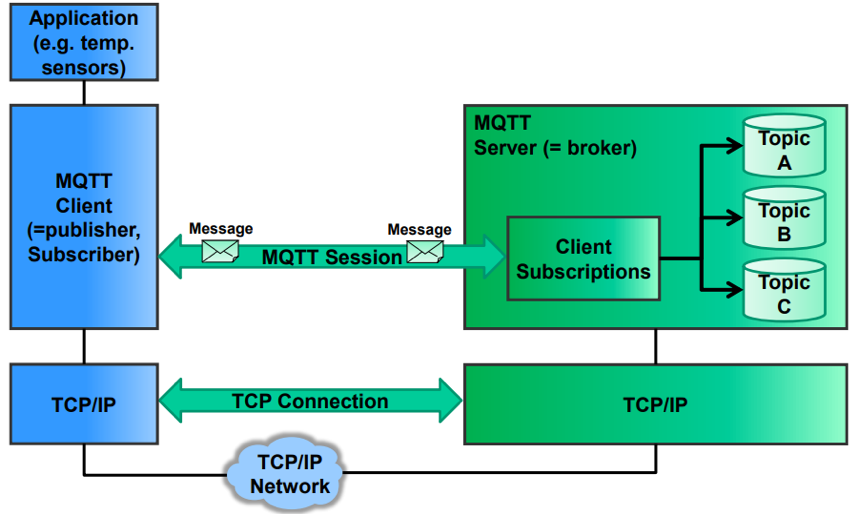
\includegraphics{mqtt_architecture}
\caption{MQTT Architecture}
\end{figure}

\bigskip
\subsection{Publish/Subscribe pattern}
\bigskip
MQTT protocol exploits the modern publish/subscribe pattern, sometimes called pub-sub, which is a valid alternative to the traditional client-server model, in which a client communicates directly with an endpoint.
This design pattern provides asynchronous communication between clients.
As you can see in the above schema, nodes are arranged around a component, usually called \textbf{broker} or \textbf{dispatcher}, in a star topology and talk to each other through it.\\
The sender of a message is called \textbf{publisher}, while who is going to receive it is called \textbf{subscriber}.\\
So, a broker is nothing but a kind of message container, known by both the publisher and subscriber, able to filter all incoming messages and distribute them accordingly.\\

\subsection{Topics and subscription}
\bigskip
Clients publish or subscribe to particular topics, which are simply message subjects having a syntax similar to URLs. For instance, assuming we want two topics related to sensors placed in our kitchen and bedroom, we may opt for the following names: $$'sensors/home/lights/kitchen'$$ $$'sensors/home/lights/bedroom'$$\\
MQTT brokers exploit these topics to decide who will receive messages, in fact if a publisher \texttt{P} publishes a message on the first topic, and a subscriber \texttt{S} subscribes to the second, this last one will not receive anything because it is not subscribed, and consequently not interested, in messages regarding the light's sensors placed in the kitchen.\\\\ 
It is important to notice that publishers and subscribers do not know about the existence of one another, but they can talk anyway.
This behaviour is part of a process called \textbf{decoupling of publisher and receiver}, which can be split in 3 dimensions:

\begin{itemize}
  \setlength{\itemindent}{+4mm}
  \item[$\bullet$] \textbf{space decoupling}: publisher and subscriber do not know each other; to be more clear, they do not know the IP address and port used by the other one
  \item[$\bullet$] \textbf{time decoupling}: publisher and subscriber do not have to be synchronized and may run at different times
  \item[$\bullet$] \textbf{synchronization decoupling}: operations on both components are not halted while publishing or receiving messages; they are independent
\end{itemize}\
In the next page, we are going to take a look at a schematic  example of the publish/subscribe pattern combined with topics subscription, but, in order to better understand it, let's keep a reference list of the existent MQTT messages we are going to deal with.


\begin{figure}[H]
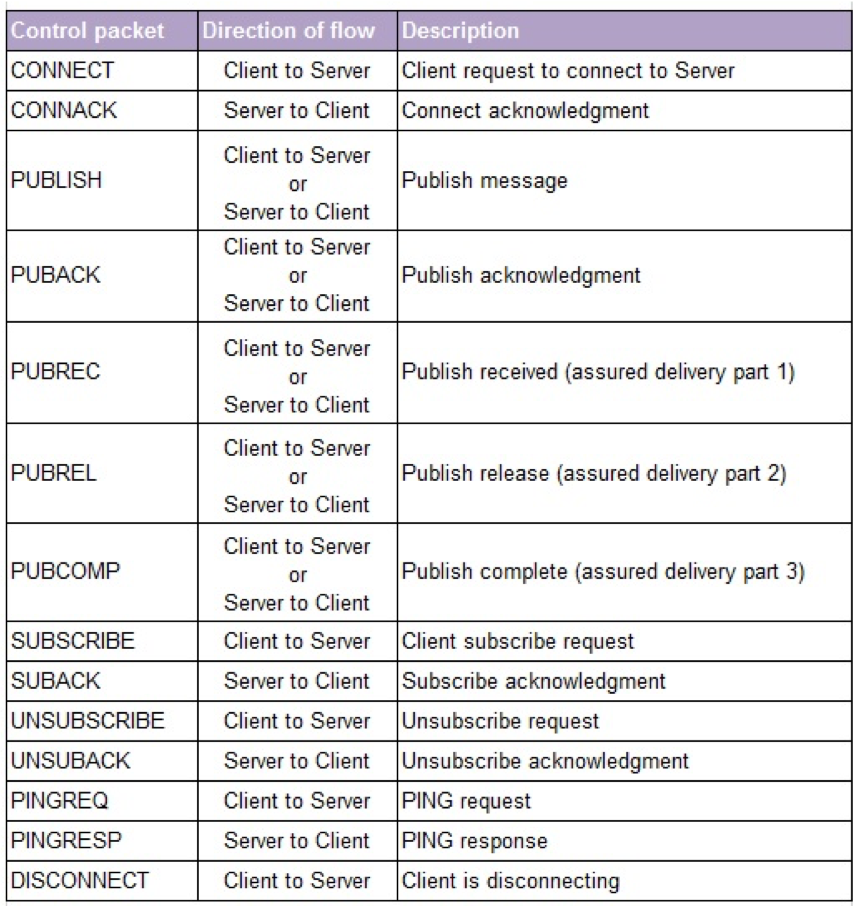
\includegraphics[width=12cm,height=13cm,keepaspectratio]{mqtt_messages}
\centering
\caption{MQTT messages}
\end{figure}

Message types' names are self-explanatory, anyway we will describe some of them more in details along the way.\\\\
Now, let's analyze the example we were talking about.

\begin{figure}[H]
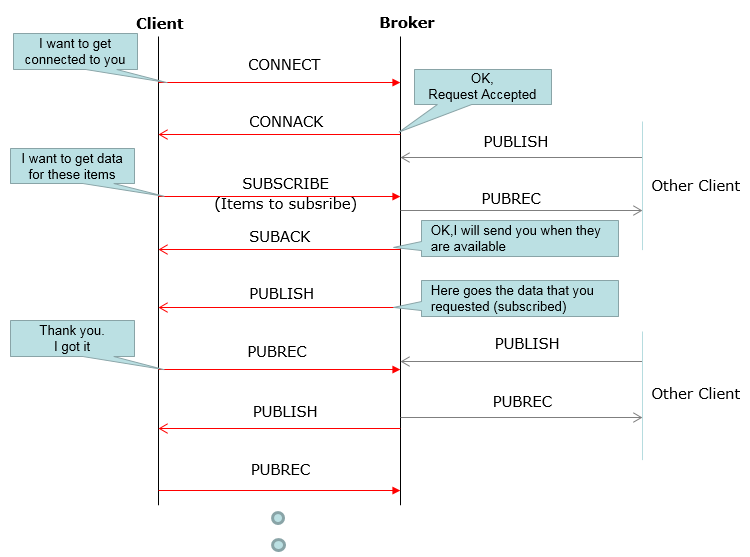
\includegraphics[width=11cm,height=10cm,keepaspectratio]{pubsub_schema}
\centering
\caption{Publish/Subscribe combined with Topics}
\end{figure}

\begin{enumerate}
\setlength{\itemindent}{+5mm}
\item A client wants to connect to the broker, and sends the proper CONNECT packet

\begin{figure}[H]
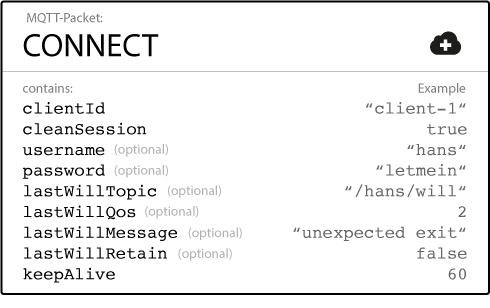
\includegraphics[width=6.6cm,height=6.6cm,keepaspectratio]{connect_message}
\centering
\caption{CONNECT packet}
\end{figure}\

where:

\begin{itemize}
\setlength{\itemindent}{+4mm}
  \item[$\bullet$] \textbf{clientId} is a identifier, unique per broker, each client must have.\\
  \textit{If you do not need a state to be hold by the broker, in MQTT 3.1.1 it is possible to send an empty value.}
  \item[$\bullet$] \textbf{clean session} is used to establish persistent connections
  \item[$\bullet$] \textbf{username} and \textbf{password} are used to authenticate the user in a password-protected broker. These credentials are sent in plain-text, therefore we will see later how to face this not neglibible problem.
  \item[$\bullet$] \textbf{keep alive} is nothing but a time interval used by the client to commit regular \texttt{PING Request} messages to the broker (this last one will reply with a \texttt{PING Response} message)
\end{itemize}

\item Once the broker has received a connection request, it replies with a \texttt{CONNACK} packet, within which there is a field called \textit{return code}, which can assume six different values, where the first one (Connection accepted) indicates the connectin has been accepted, while the remaining ones indicate that connection has been refused for some reason (Unacceptable protocol version, Invalid identifier, Server unavailable, Not Authorized, Bad username and password)

\item Assuming that the connection has been accepted by the broker, then the client can choose to publish a message or subscribe to a topic.\\\\
In the first case it will send a \texttt{PUBLISH} packet

\begin{figure}[H]
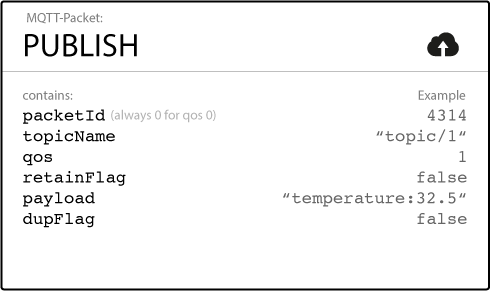
\includegraphics[width=6.6cm,height=6.6cm,keepaspectratio]{publish_message}
\centering
\caption{PUBLISH packet}
\end{figure}\

where:

\begin{itemize}
\setlength{\itemindent}{+4mm}
\item \textbf{packetId} is a reference id to the current packet
\item \textbf{topicName} is the topic we want to publish on
\item \textbf{qos} and \textbf{retainFlag} will be explained in details in a few pages
\item \textbf{payload} simply represents the content of the message
\item \textbf{dupFlag} is a flag used to warn who receives the message that this message might have been already received
\end{itemize}

The broker will reply sending a \texttt{PUBREC} packet, used to let the client know that its message has been received correctly.
\bigskip \\
In the second case it will send a \texttt{SUBSCRIBE} packet, which contains multiple pairs \textit{(topic,qos)}, since a single packet can be used to subscribe to multiple topics.\\
Clearly, the broker will reply with a \texttt{SUBACK} packet, containing the return code for each topic the client is interested to.

\item If a client wants to unsubscribe a topic it simply sends an \texttt{UNSUBSCRIBE}  packet to the broker (as in the SUBSCRIBE case, the client can specify multiple topics).

\item Finally, the user should disconnect gracefully from the broker sending a \texttt{DISCONNECT} message.\\\\\\

\end{enumerate}
\bigskip

{\setlength{\parindent}{0cm}
Now that we have an idea of how MQTT communications work, in the next page we are going to see quickly some protocol's aspects regarding the quality of the service.
}

\clearpage

\subsection{Quality of Service Levels (QoS)}

\bigskip
Previously, we have briefly introduced the structure of the \texttt{PUBLISH} and \texttt{SUBSCRIBE} packets; both of them contain a field called \textbf{QoS}, acronym of \textbf{Quality of Service}.\\
This field allows clients to set the desired QoS level, according to how much reliability they expect from message delivering.
Clearly, being QoS level an agreement between the client and the broker, this last one has to honor the contract.
There exist three different QoS levels:

\begin{itemize}
\setlength{\itemindent}{+4mm}
\item \textbf{QoS0 (at most once delivery)}: messages are sent at most once, besides their delivery is not guaranteed
\item \textbf{QoS1 (at least once delivery)} messages are certainly delivered to the client at least once, but they might be also delivered more times.
\item \textbf{QoS2 (exactly once delivery)} messages are sent exactly once by using the following 4-way handshake mechanism.

\begin{figure}[H]
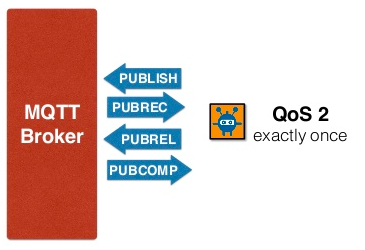
\includegraphics[width=6cm,height=6cm,keepaspectratio]{mqtt_qos2}
\centering
\caption{MQTT QoS2 4-way handshake}
\end{figure}
Of course, the exchange of 4 packets increases the overhead and afflicts performances, therefore this level should be used only in critical scenarios that cannot afford to lose messages or receiving duplicated messages.\\

\end{itemize}

{\setlength{\parindent}{0cm} {The following real-world examples help to better understand when we should choose one level rather than the others.\\
}

\begin{itemize}
\setlength{\itemindent}{+4mm}
\item \textit{if we have a series of solar panels that publish every second some measures on a specific topic, we can accept with no worries that some messages are not delivered correctly, so we may think to use QoS0.}
\item \textit{if we have an alarm sensor which publishes an alert message on a topic only if something bad happened in our house, then we want to be sure that such message will be correctly delivered, even more than once, so we may opt for QoS1.}
\item \textit{in this last scenario, we assume that for some reason there is a diabetic person having an auto-injecting insuline device applied to his body, which expects to receive an MQTT message when an extra injection is needed.\\Obviously, in this case it is necessary to receive one and only one message, so we must choose QoS2.}
\end{itemize}

\bigskip
\subsection{Retained messages}
\bigskip
In MQTT, a retained message is a normal message having the retained flag set to true.
MQTT brokers always store the last retained message received, in order to send it to new subscribers, immediately after subscribing to the related topic.\\\\
What are retained messages useful for?\\

We must remember that MQTT clients are autonomous, therefore they do not know the presence of each other; this means that when a subscriber subscribes to a topic, it has no way of discovering how much time it will take before receiving a message.\\
This problem is solved using retained messages.\\

Example scenario: \\

\textit{if we have a certain device which updates his online status (true/false) on the topic '/devices/devicename/status' only when it changes, and a new subscriber arrives, then he would probably want to be notified immediately about the status of the device.}

\subsection{Persistence}
\bigskip
MQTT also supports persistence of messages.\\
This feature is very useful because each time a client connects to the broker, a new session for subscribing or publishing to topics is started; if, for any reason, the connection is lost, the process starts all over again with the client establishing a new session.\\
Clearly, this behaviour afflictis the performances of the system, especially when clients have low power and poor connectivity (for instance, intermittent connectivity).\\
Let's notice an important aspect of this feature that we are going to discuss later: to resume a session, the broker has to recognize the user to be the same as before, and it is able to do that by using its unique identifier; once the broker found the match between the clientId and an available persistent session, that session is immediately reassigned to the client.\\

\subsection{Last Will and Testament (LWT)}
\bigskip
It is not uncommon for clients to get disconnected ungracefully from the broker.\\
There exist scenarios in which it may be helpful to notify other clients that a specific client has been suddenly disconnected.\\
Thanks to the LWT feature provided by MQTT brokers, clients can choose a message that will be published to previously chosen topics when they get disconnected.\\
As already seen previously, the client can specify the LWT message as part of the \texttt{CONNECT} packet, then the broker will store the message till it detects that the client has been disconnected badly, finally topic's subscribed clients will be notified.\\
Let's clarify that saying "ungracefully disconnected" means that a network failure happens, or the client fails to communicate within the keep-alive time, or the client closes the connection without sending a \texttt{DISCONNECT} message or the server faced a protocol error.\\\\
In the real world LWT is often used in combination with retained messages to keep updated the state of a client on a specific topic.\\
For instance, when a client has connected to a broker, it will send a retained message to a topic, named something similar to \textit{"clientname/status"}, with the payload \textit{"online"}.
After that, the client sets the LWT message on the same topic to \textit{"offline"} and, clearly, mark it as retained.



\chapter{Security Overview}

\section{Introduction}
\bigskip
MQTT is probably the most used IoT protocol, and experts think it will play an important role in the coming years, therefore it is necessary to take about its security aspects.\\
Just to begin, we can take a look at this real-world example in order to understand how much used this protocol is, but how many times its security is completely ignored.\\\\
In this example we are going to use a search engine, called \textbf{Shodan}.\\
Shodan, developed in 2009, lets the user find specific IoT "things"(webcams, routers, servers, sensors, printers, traffic lights, etc)  connected to the Internet, providing a huge variety of filters.\\

Thanks to its dangerousness and power, many people call it \textit{"the hackers' search engine"}.\\
Its searching mechanism is based on the so-called \textit{service banners}, which are nothing but metadata sent back to clients by servers: service banners contain a lot of information describing the kind of server/device you are talking to.\\

By default, MQTT brokers listen on port 1883; said that, we can simply find the current visible servers listening on that port by using Shodan and its filters, searching for \textit{"port:1883"}.\\\\
This is what we obtain:\\

\begin{figure}[H]
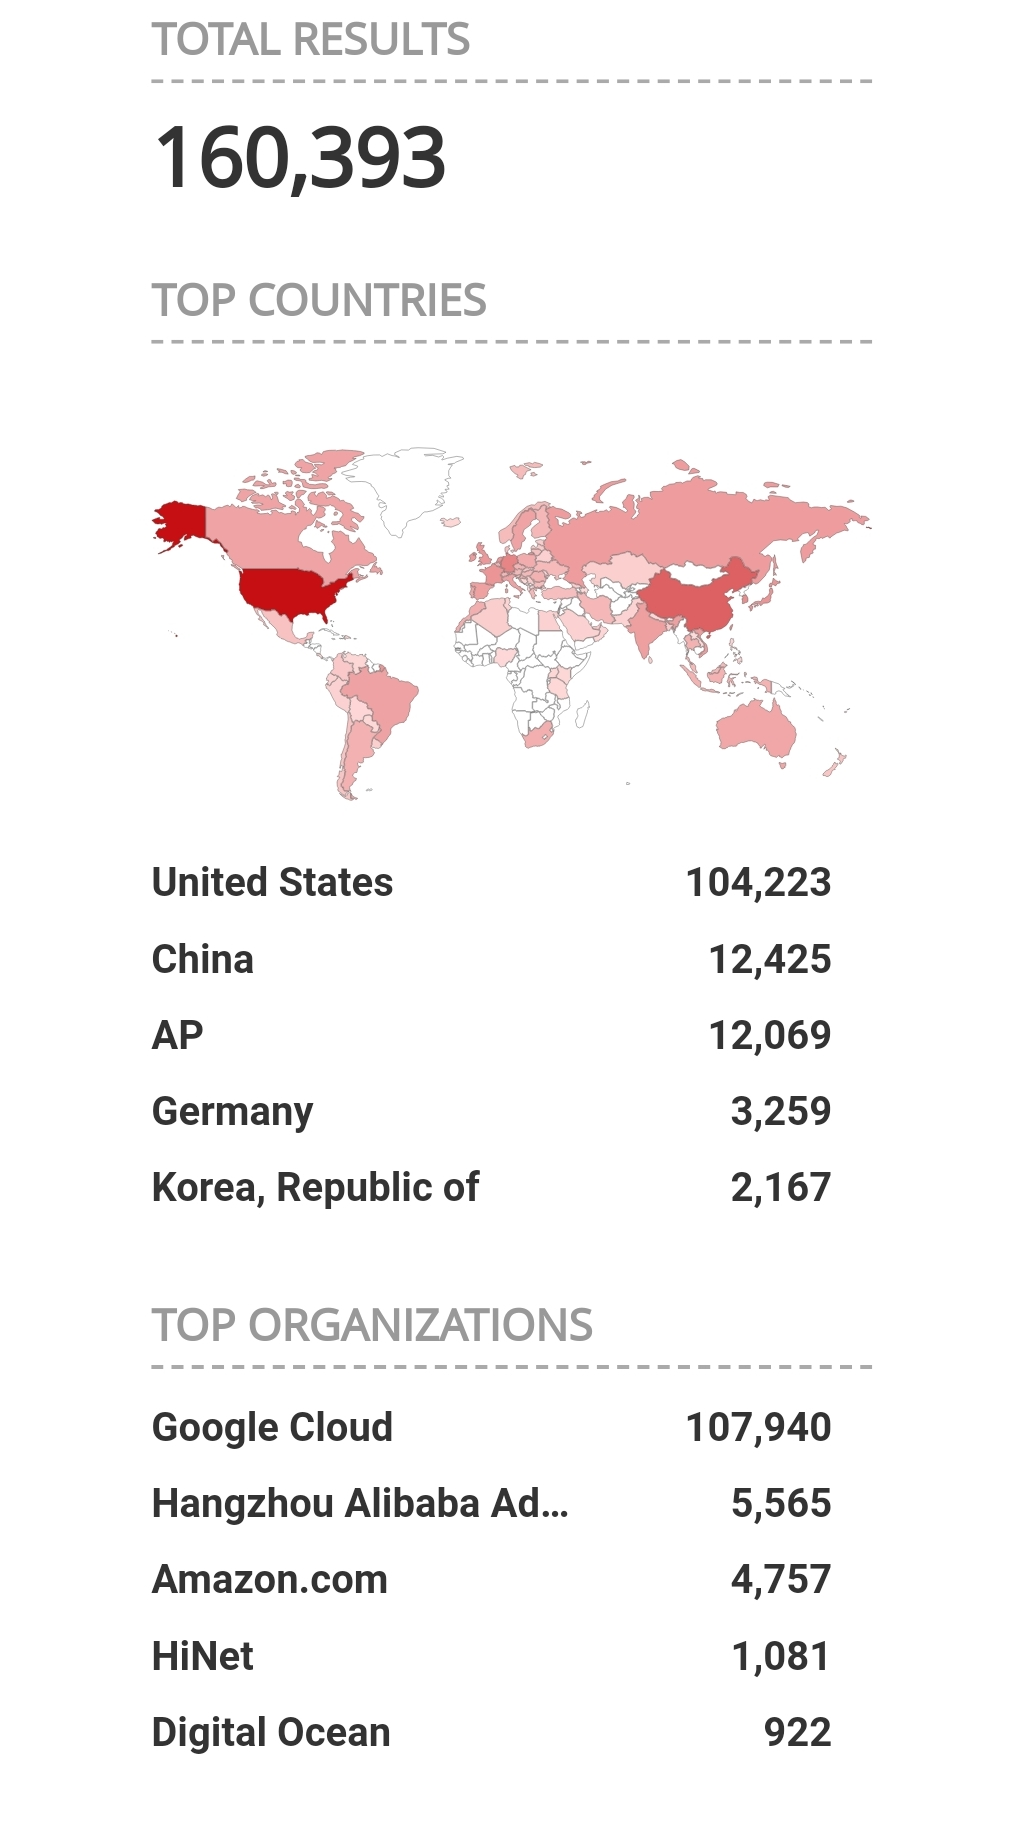
\includegraphics[width=9cm,height=9cm,keepaspectratio]{shodan_numdevices}
\centering
\caption{MQTT brokers found using Shodan}
\end{figure}\

We found, all over the world, more than 50 thousand devices listening on port 1883, many of them owned by important organizations like Amazon, Microsoft and Alibaba.
This is just a big number, but the more interesting thing is that this number is growing up very quickly: just to realize, two weeks ago the same research gave me 46 almost thousand devices.\\\\
The port 8883 is standardized for a secured MQTT connection, whose name is "secure-mqtt", and this port is exclusively reserved for MQTT over TLS.
The first proof that lead us to think that security is neglected is that, if we search again on Shodan, this time filtering on port 8883, we get only 56 servers, so stastically only one broker in a thousand opt for the secure version of the protocol.

Besides, I found a very interesting article on a reliable blog I have been visiting for several years, whose content is strongly related to cyber security.\\
An easy-to-implement Python scanner script, exploiting a paid Shodan API key, has been implemented to search for servers listening on port 1883 and then try to connect to them sending a \texttt{CONNECT} message with no authentication.
The strategy of this attack is pretty simple: the broker we are trying to connect to will reply, as we have already seen, with a \texttt{CONNACK} packet containing the return code; if the return code is equal to 0 it means that the connection has been accepted, therefore the broker leaves the door open to anyone.\\
An analysis conducted on 800 found servers, has led to the following results.

\begin{figure}[H]
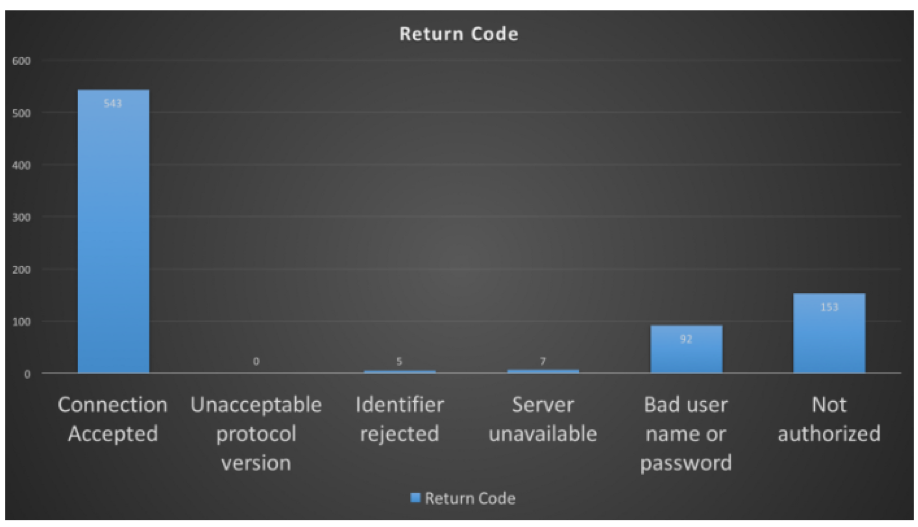
\includegraphics[width=9cm,height=9cm,keepaspectratio]{shodan_results}
\centering
\caption{MQTT brokers return code stastistics}
\end{figure}\
543 brokers out of 800, which is almost 67\%, do not use authentication at all!
\\\\\\\\
Now that we have realized how much MQTT security is neglected in real-world applications, let's start talking in details about this fundamental aspect.

\clearpage

\section{MQTT combined with TLS}
\bigskip
Before starting to talk about the authentication methods used by MQTT, we must always remember that MQTT relies on TCP as transport protocol, which means that by default the protocol itself has no built-in encryption.\\
This choice was made purposely by developers to keep it simple, fast and lightweight; therefore, everything is sent in plain text.\\\\
We know that TLS uses an handshake mechanism to negotiate various parameters necessary to establish an encrypted and safe communication which cannot be read or altered by third parties.\\
Usually what happens is that servers provide their \textit{X.509 certificates}, signed by a trusted authority, to clients to prove their identity.\\
The negotiation of the parameters brings to a communication overhead afflicting performances.\\
This overhead brings devices' CPU to do more work than before and this may turn out to be a problem for very constrained devices.\\
Let's suppose to have a constrained device which establish a new connection every time it has to communicate with the broker; this will bring a huge overhead because the handshaking messages are quite heavy and will be the most significant portion of content to send in each communication (considering that usually mqtt devices send simple text messages of few bytes, and the handhsake ones a few KB).\\
Therefore it is recommended for constrained devices to use long-living MQTT connections rather than short-living ones in order to drastically improve the TLS performances; based on this idea there exists a technique, called \textbf{Session resumption}.

\subsection{Session resumption}
\bigskip
The idea is pretty simple: TLS session resumption techniques allow to reuse an already negotiated TLS session after reconnecting to the server; doing this way the client does not have to perform the entire TLS handshake again.\\
Unfortunately, some TLS libraries do not implement session resumption techniques, but most of them do it.\\\\\\
There exist two session resumption techniques:
\begin{itemize}
\setlength{\itemindent}{+4mm}
  \item[$\bullet$] \texttt{Session Ids}: the server simply stores the secret Session Id associated to a client, so that when this last one reconnects, it provides the Session Id and the session is resumed.
  \item[$\bullet$] \texttt{Session tickets}: the servers send to the client a secret ticket encrypted with a secret key known only by the server.\\
  When the client reconnects, it sends its state to the server and if this last one is able to decrypt it, the session is resumed with the state contained in the secret ticket.
\end{itemize}\
Despite everything, very constrained devices do not have enough computational power to support TLS anyway. 
In this case, clients might think to use TLS-PSK cipher suites (not supported by all TLS libraries), since they avoid CPU intensive operations, or totally avoid TLS and use other strategies we are going to discuss later.\\\\

To conclude this TLS section, we can list some best practices:

\begin{itemize}
\setlength{\itemindent}{+4mm}
  \item[$\bullet$] Clients should always use TLS or, more generically, encrypted communication channels, if they can afford it
  \item[$\bullet$] Use the newest version of TLS, because older ones might have known, and now fixed, bugs
  \item[$\bullet$] Do not use SSLv3 or any prior versions, they are broken. There are many dangerous vulnerabilities came out in the last years, and a simple example is Heartbleed
  \item[$\bullet$] Always use certificates from trusted Certification Authorities. Using self-signed certificates or allow-all approach is not recommended
  \item[$\bullet$] Including additional security mechanisms, like payload encryption and authorization mechanisms, in addition to TLS is a good choice.

\end{itemize}\

In the next section we will talk about client authentication techniques supported by MQTT.


\section{Client Authentication}
\bigskip

There are 3 ways used by MQTT brokers to verify the identity of a client:

\begin{itemize}
\setlength{\itemindent}{+4mm}
  \item[$\bullet$] Client Id
  \item[$\bullet$] Username and Password
  \item[$\bullet$] X.509 Client certificates
\end{itemize}\

Let's analyze each of them in details.\\


\subsection{Client Id}
\bigskip
We have already seen that clients must include within the \texttt{CONNECT} message a field called \textit{clientId} to identify themselves.\\
This procedure can be, in some way, already considered as a form of authentication since each client must have a unique identifier.\\
It is common practice to use 36-character long identifiers, or some unique information available to the client like his MAC address, or the serial number of the device.
Clearly, this is not safe because someone can easily pretend to be you, just by connecting to the broker specifying your clientId.\\
Depending on the broker's configuration, if the real client has already connected to the broker, the attacker's connection request would be discarded or the real client would be disconnected, but if not, the connection would be certainly accepted.\\

How can the attacker obtain this information? He can easily sniff that, since communication is not encrypted.\\

Moral of the story: \textbf{never rely on clientId to secure our system}.\\

\subsection{Username and Password}
\bigskip
There are two main problems related to this authentication method:

\begin{itemize}
\setlength{\itemindent}{+4mm}
  \item[$\bullet$] Since, by default, no encryption system is used, using credentials is totally pointless, in fact even a trivial MITM attack would be enough to sniff them without effort, as we can see in the image below.

\begin{figure}[H]
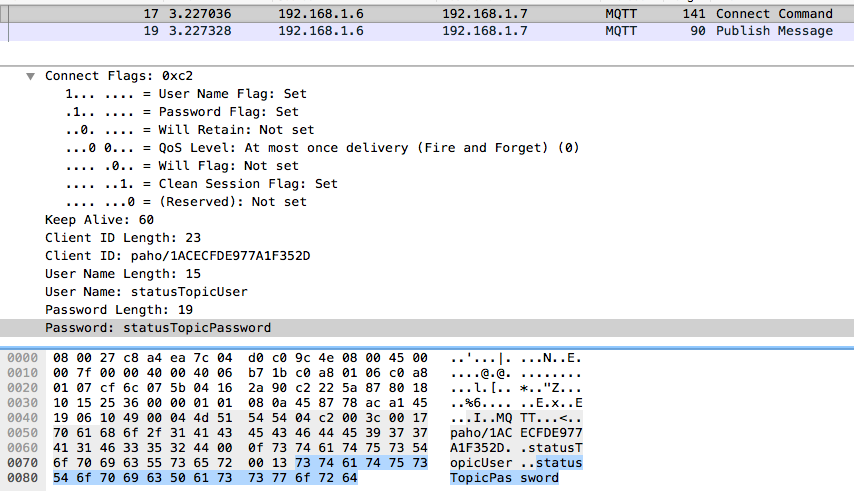
\includegraphics[width=11cm,height=11cm,keepaspectratio]{wireshark_credentials}
\centering
\caption{MQTT credentials sent in plain text}
\end{figure}

\item[$\bullet$] Authentication is optional, so a huge number of topics are easily accessible from the whole world.\\

The only way to use credentials safely is to combine them with an encrytped communication (better if TLS).

\end{itemize}

\subsection{X.509 Client certificates}
\bigskip

Another possible way to identify clients is using their X.509 certificates, which will be sent during the TLS handshake.\\
We are used to servers providing their X.509 certificates to clients to prove their identity, and clients authenticating in the application layer.\\
In this case, instead, we talk about mutual authentication, since client and server authenticate each other at the same time using X.509 certificates.\\
This authentication method is very secure but rarely used because it requires the provisioning and managing of the certificates to the clients, besides this double negotiation afflicts even more the performances.\\

Now, let's take a look at pros and cons of using client certificates.
\begin{itemize}
\setlength{\itemindent}{+4mm}
\item[$\bullet$] Pros:
\begin{itemize}
\item only valid clients are allowed to establish a secure connection
\item authentication of clients at transport level, so invalid clients are discarded before \texttt{CONNECT} messages are sent.\\ this is very useful to save resources on broker's side, because authentication mechanism can be expensive (a common case is that credentials are stored in a database which must be interrogated every time someone wants to connect) and using client certificates makes them useless and, therefore, avoidable since authentication is done before a connection is established.
\end{itemize}

\item[$\bullet$] Cons:
\begin{itemize}
\item Managing a huge number of client certificates may be a serious problem, therefore it is important to have a solid certificate provisioning process: in other words, clients' certificates must be kept updated, and owners should have a way to manage their lifecycle: if they are able to control all their MQTT clients, making possible to update their certificate periodically, it is suggested to use certificates, but if the clients are not under their strict control, then it is not recommended to use them.
\item It could happen that a client's certificate get leaked and, consequently, cannot be trusted anymore since some attacker uses it, so it it necessary to have a way to revoke invalid certificates.\\
There are two ways to obtain that:

\begin{enumerate}
\item \textbf{Publish Certificate Revocation Lists (CRLs)}: they are simple lists of invalid certificates.
Servers are able to recognize invalid client certificates consulting their list; clearly, servers has to exchange their lists in order to stay up to date. This is not a very convenient procedure.
\item \textbf{Online Certificate Status Protocol (OCSP)}:  it is a protocol used for asking information about specific client certificates, more in details to know if they are still trustable.\\
In order to use OCSP there must be a so-called \textit{OCSP Responder}, which is an HTTP server waiting for revocation-check requests, provided by the certification authority.
This is a better and faster solution since you do not have to communicate with other srvers to stay up to date; you simply ask your certification authority, which is going to do the boring job for you.\\
Let's see a simple example of how it works:

\begin{itemize}
\item Alice and Bob want to communicate and have their certificates issued by a certification authority, called Carol
\item Alice starts the transaction by sending to Bob her certificate
\item Bob, who suspects that Alice's private key might have been compromised, sends an \textit{OCSP request}, containing Alice's certificate serial number, to Carol
\item Carol's OCSP responder search in its database the certificate's serial number received from Bob
\item At this point, Carol's OCSP responder returns a signed successful \textit{OCSP response} to Bob if the certificate is still valid, otherwise will reply telling Bob that the certificate is not valid anymore
\item Depending on the response received by Carol, Bob will carry on, or not, the communication with Alice.\\
\end{itemize}


\end{enumerate}
\end{itemize}
\end{itemize}


Conclusion: This kind of authentication is safe but expensive, therefore only suited to a small number of clients which needs an high security. \\

In the next section we will discuss about authorization, another important concept related to security which is, even if does not seem to, different from authentication.\\


\section{Authorization}
\bigskip
Authorization and authentication go hand in hand, but they are very different security concepts.\\
While authentication is used to recognize the identity of a client, authorization allow us to create policies in order to restrict access to certain resources (\textbf{in this scenario resource means topic}).\\
We can better understand this concept with an example related to web applications:\\

\textit{Talking about Facebook, let's suppose to have a standard user and a developer.
When we visit Facebook, we are asked to insert username and password to let the application identify us and this is the authentication part, equal for everyone.
Then, the authorization process is different for the two users, in fact the standard user will have a more restricted access to resources, compared to the developer.}\\

Coming back to MQTT, let's try to understand which constraints can be applied to clients.\\
A client, once connected to a broker, can publish messages and subscribe to topics, nothing more.\\
We may notice that without authorization every authenticated client could do whatever he wants, so publish or subscribe to any existent topic.\\
More in details, the resources to protect are the common actions: publishing, subscribing, setting a LWT message, requires a persistent session.\\\\
How can the broker restrict permissions on topics?\\

Brokers can limit clients permissions implementing some authorization policies called \textbf{topic permissions}, having, at least, the following information:

\begin{itemize}
\setlength{\itemindent}{+4mm}
  \item[$\bullet$] Allowed topic
  \item[$\bullet$] Allowed operations (publish, subscribe, LWT, retained messages)
  \item[$\bullet$] Allowed quality of service levels (0, 1, 2, all)
\end{itemize}

What does it happens when a client tries to access a restricted resource without having enough permissions?\\

If the client tries to publish, the broker can disconnect it or simply reply to it normally, but not sending the message to subscribers; instead, if the client tries to subscribe, the broker will reply with a standard \texttt{SUBACK} message containing a proper return code which tells the client that its subscription was denied, nothing more.\\

In the next section we are going to discuss about another form of authentication/authorization mechanism usually implemented in other protocols, like HTTP, and we will see wether and how it is possible to combine it with MQTT. 

\section{MQTT combined with OAuth 2.0}
\bigskip
OAuth is a standard for access delegation, used to allows a third party to access a resource owned by a resource owner without giving unencrypted credentials to the third party.

\begin{figure}[H]
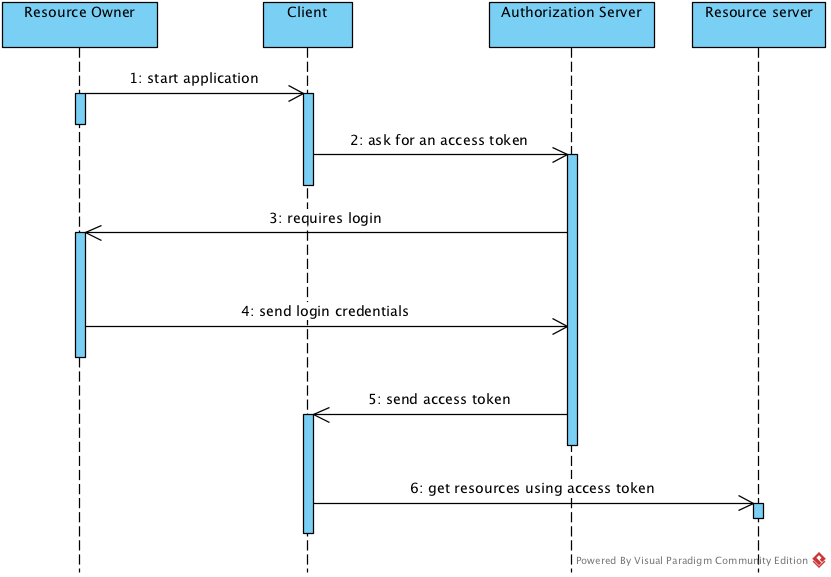
\includegraphics[width=11cm,height=10cm,keepaspectratio]{oauth_scheme}
\centering
\caption{OAuth working scheme}
\end{figure}

To make it clear, we may think to Spotify which allows its users to login with their Facebook account, then once they have authenticated, it gets their information (resources), like name, surname and maybe something else, from Facebook resources server.\\
More in details, referring to the above schema, we have that Spotify is the client, Authorization server is the Facebook Authorization server, in charge to control the access to all the resources, and the Resource server is the Facebook Resource server where there are contained the information Spotify is going to take.\\
The resource owner (the user) will login on Facebook communicating directly with its Authorization Server, without giving any credential to the client. Once Facebook authenticated the resource owner, it sends the access token to the client.

So, the idea is pretty simple: we do not want to save our credentials within the client and use them every time to authenticate us because it could be dangerous, therefore the solution is using access tokens.\\
Clearly, if we do not use encrypted communications everything is pointless because an attacker could easily sniff our access tokens and use it to access our own resources.\\

What is the token's structure?\\

Usually, OAuth uses \textbf{JSON Web Tokens (JWT)}, JSON Objects with base64 encoding. They contain header, payload and signature, where:

\begin{itemize}
\setlength{\itemindent}{+4mm}
  \item[$\bullet$] The header contains information about the algorithms used to encrypt and sign
  \item[$\bullet$] The payload contains information about the token, like expiration date, scope, issuer, issue date, etc.
  \item[$\bullet$] The signature is used to certify that the token has been signed by the trusted authorization server
  \end{itemize}

How can we exploit this standard in MQTT?\\

First of all, we have to clarify that OAuth is mainly designed for usages with HTTP, so over any other protocol is out of scope, but we can analyze the possible MQTT workarounds.\\
We notice that in the previous example, the login to the authorization server expects a human action, but IoT are often standalone, therefore no human can help them in this OAuth authentication process; they have to be both the client and the resource owner, but this is against the OAuth principles since it was born to avoid clients to hold their credentials locally.\\\\
Anyway, since IoT devices are standalone, this is the only way to use OAuth: storing the credentials within the devices, use them to get a valid access token from an Authorization Server, finally use it to communicate with the broker.\\Obviously, the access token must have a not too small expiration time, because if so the client should ask for the token every time it wants to communicate with the broker, but this would be equivalent to send once the username and password to the broker at the beginning of the communication.\\

Probably, the real pros of using tokens in MQTT is that they can be used to get client's authorizations quickly, saving search time to the server: if no token is used, the broker will have to look up for users' authorizations in a database (after its authentication); a faster and more convenient way is to specify the permissions granted to the client within the token (for instance, in the payload). \\
This way is safe, because, as already said, the broker is able to verify the authenticity of the token thanks to its signature.

The access token will be used in \texttt{CONNECT} packets, and optionally in \texttt{PUBLISH} and \texttt{SUBSCRIBE} ones. Before making this last decision, since there are tons of pub/sub messages, it is important to consider how much token validation afflicts performances, and, if necessary, think to some caching method.\\\\

Conclusion: OAuth is a valid authentication mechanism, but it is difficult to combine with MQTT; besides, before deciding wether to use it or not, it is fundamental to evaluate if the few advantages obtained are worth the effort of implementation.


\section{Simple Data Encryption}
\bigskip
We have already said that some devices have too low power to use TLS.
In this section we are going to discuss how constraint devices may think to encrypt only specific data, like the payload in the \texttt{PUBLISH} message, or credentials within the \texttt{CONNECT} packet, and pros and cons of doing that.\\
Using this strategy we will have sensitive data, let's assume the payload in our examples, will be encrypted, but other metadata remains untouched.\\
Let's notice that the broker has no key to decrypt the encrypted data, so it will send the message to subscribers as is, without knowing its real content.\\
Clearly, this mechanism expects subscribers to have the proper key to decrypt the encrypted message received by the broker.\\
The following schema explains this scenario, called \textbf{End-to-End}, perfectly.

\begin{figure}[H]
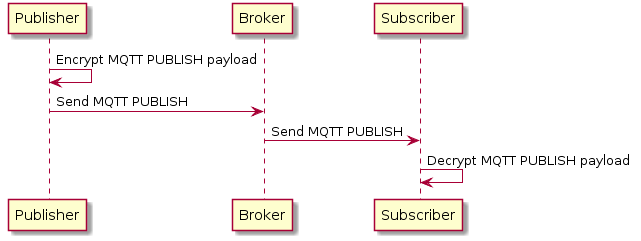
\includegraphics[width=12cm,height=12cm,keepaspectratio]{end_to_end}
\centering
\caption{MQTT communication using End-to-End encryption}
\end{figure}

Now, a question arises: if we are going to encrypt other data, like client's credentials in the \texttt{CONNECT} packet, how can the broker decrypt and validate them?
This is a very uncommon and boring practice, because it is necessary to write an additional plugin for the broker we are going to use in order to make it able to decrypt our data. 
This second scenario is called \textbf{Client-to-Broker}.\\
In this case, the broker will send the decrypted message to subscribers, which will not have to know any key.

\begin{figure}[H]
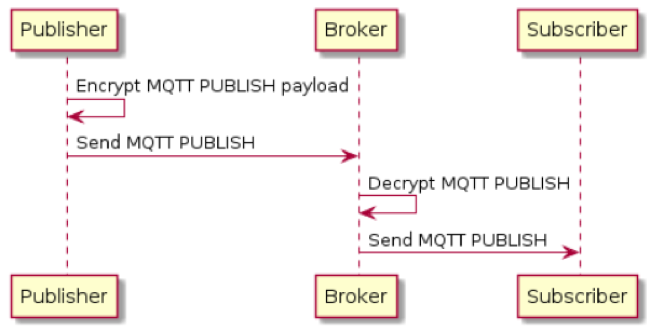
\includegraphics[width=10cm,height=10cm,keepaspectratio]{client_to_broker}
\centering
\caption{MQTT communication using End-to-End encryption}
\end{figure}

As we know, there exist asymmetric and symmetric encryptions. Which one should we opt for encrypting payload in a \texttt{PUBLISH} message?

\begin{itemize}
\setlength{\itemindent}{+4mm}
  \item[$\bullet$] we should prefer asymmetric one if we have many publishers and a few trusted subscribers, because these last ones know the private key, so they can read all the messages in the subscribed topic
  \item[$\bullet$] we should use symmetric one if we have a trusted environment, in fact we must remember that in this case there is only one key to encrypt and decrypt, so we cannot share it with everyone.
\end{itemize}
\bigskip
Certainly, using symmetric key is simpler to implement, but it is more limited talking about usability.

We conclude this section wrapping up the pros and cons of data encryption:

\begin{itemize}
\setlength{\itemindent}{+4mm}
\item encrypting specific data adds a security layer to communication and can be an option for constrained devices which cannot rely on TLS
\item[$\bullet$] even if TLS is heavier, encrypting and decrypting every message can be intensive for constrained devices, in fact it is fundamental to choose a fast encryption algorithm
\item[$\bullet$] we must remember that encrypting only specific data prevents attackers to sniff our sensitive information, but man in the middle attacks, as well as replay attacks, are still possible.\\ 
Just to make an example: an attacker could intercept a valid message and modify some parts of it, like the topic
\item[$\bullet$] It may be difficult to work properly with keys, for instance it is important to establish a secure provisioning of them.
\end{itemize}
\bigskip
In the next section we are going to see another fundamental security aspect different from secrecy, which is data integrity.\\

\section{Data Integrity}
\bigskip

Previously we talked about tokens and how their signatures are used to make sure they have been generated by a trusted source, like the Authorization server; now, let's see, in general, how brokers can validate received messages.\\
Data integrity checks is fundamental because it is the only way to assert that the content of a message is authentic and has not been altered by third parties.\\
There are 3 different approaches for message integrity checks:

\begin{itemize}
\setlength{\itemindent}{+4mm}
\item[$\bullet$] \textbf{Checksum}: a value calculated, with a series of calculations that converts the message payload into a string of digits, which is usually called \textit{hash}.\\
This hash is simply attached at the beginning of the payload, so the receiveing application has just to recalculate the checksum to verify the integrity of the message.\\
This approach guarantees that data was not modified, but it is not able to assure that it comes from a trusted sender, since there is not key involved.

\item[$\bullet$] \textbf{Message Authentication Code (MAC)}: this authentication code needs a MAC algorithm able to generate a MAC starting from a secret key and the message payload.\\
Then, the client sends the message including the generated MAC.
Clearly, the receiving application must know the same secret key that was used to generate the MAC, in order to validate it.\\
This approach guarantees that data was not modified and also that it comes from a trusted sender.\\
We notice that the secret key is the same for all the clients, so using MACs we are not able to guarantee non-repudiation.

\item[$\bullet$] \textbf{Digital signature}: it is a code generated by a public key encryption algorithm. More in details, the client signs the message with its private key and the broker validates the signature using the public key of the client.\\
The public key can be included in the MQTT message sent by the client.\\
This approach is the most secure because is the only way to sign a message properly is knowing the private key, which is known only by the real client, but at the same time the broker has not to know it too.\\
So, this approach guarantees the same things of the previous one plus the certainity that a sepcific user sent the message.\\
The difference between the previous approach is that the secret key was shared to all clients, while in this case each client has its own private key, but the broker is still able to decrypt their messages using the public key it received.\\
\end{itemize}

Integrity checks is always a good choice: secrecy combined with integrity gives the system a robust security: secrecy prevents attackers to see our things, and integrity prevents attackers to alter them without being discovered.\\\\
In the next section, we are going to see how to make a MQTT system even more secure by using a not very common, as well as powerful, security architecture, called \textit{Software Defined Perimeter}, or simply \textit{SDP}.\\


\section{MQTT combined with an SDP}
\bigskip
In this section we will see a sophisticated solution to implement a very secure MQTT system; since this architecture's implementation seems to be a bit difficult, it should be taken into consideration only if your system needs to be extremely protected.\\

\subsection{What is an SDP?}
\bigskip
An \textbf{SDP (Software Defined Perimeter)}, also known as \textbf{Black Cloud}, is an emerging security architecture, a bit difficult to implement and manage, that restricts accesses and connections among allowed devices.\\
Once, companies used to define a local physical network perimeter in order to protect their applications from external threats.\\
Nowadays, digital progress has significantly broadened these boundaries, and IoT is the biggest proof of that, in fact having sensors scattered in different places of the world makes impossible to define a local physical network as it used to be.\\

SDP relies on a strategy based on \textit{"hidden-resources"}, or \textit{"non-visibility"}, to provide secure access to devices and applications.\\
A traditional internal network separated by the external world has a well-defined perimeter and makes use of some firewall functions denying the access to external users, but allowing internal ones to communicate with the external world.\\
Instead, an SDP is a scalable solution able to provide a secure and authorized access to resources in a perimeter in continuous evolution.\\

\textit{We may think to a network protected by an SDP like a private and exclusive society distributed all over the world, where everybody would like to access, but to which only authorized persons will access.}\\\\
It is important to say that SDPs are not strictly connected to IoT technologies, but they can be used in different fields.\\

\subsection{How does an SDP work?}
\bigskip

What happens pratically is that devices trying to access are first identified, then, once they have been accepted within the protected network, they are subjected to a further verification process, an authentication with credentials, and finally are assigned permissions based on their authorizations.\\
Let's see more in details how it works.\\

First of all, an SDP expects a secure connection, therefore encrypted, based on a \textit{"need-to-know"} logic, that allows only identified, authenticated and authorized clients to access network resources.\\
There exist many different SDP structures, as we will see in minutes, but they all refer to the idea of \textbf{"hide to protect"}.\\

The following is an example of a possible SDP structure:

\begin{figure}[H]
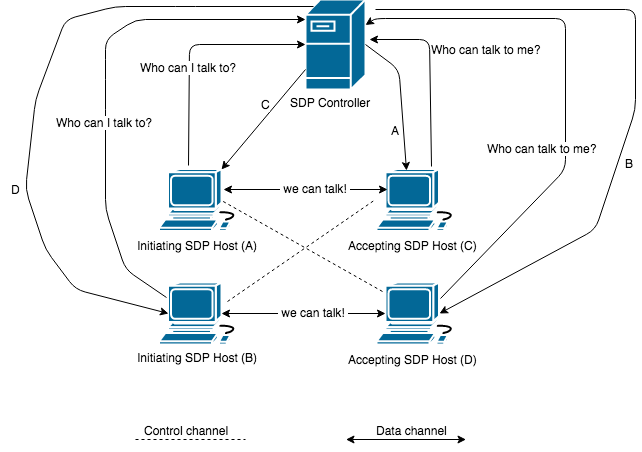
\includegraphics[width=10cm,height=10cm,keepaspectratio]{sdp_structure}
\centering
\caption{Example of  SDP structure}
\end{figure}

There are two components: \textit{SDP Hosts} and \textit{SDP Controllers}; SDP Hosts can either initiate or accept connections, and these actions are managed by interactions with the SDP controllers through a control channel.\\
This is a possible SDP workflow:

\begin{enumerate}
\item One or more Controllers are brought online and connected to the appropriate authentication/authorization services
\item Hosts, after being brought online, connect and authenticate to the controllers and, for the moment, they do not accept to communicate with any other host
\item Controllers determine a list of Accepting Hosts to which the Initiating Hosts are authorized to communicate
\item Controllers instruct the Accepting SDP Hosts to accept communication from the Initiating Hosts and gives these last ones the list of Accepting Hosts.\\
Since we said that communication is encrypted, policies containing infomation about encryption are sent to both Accepting and Initiating hosts.
\item Now Initiating Hosts can communicate with Accepting Hosts.\\
\end{enumerate}

\subsection{How can this architecture be combined with MQTT?}
\bigskip
Before describing how we can make SDP working with MQTT, let's clarify that the SDPs we are going to see are not exactly like the above one: they are similar, since they follow the idea of "hide to protect", but simpler.\\

We have seen that MQTT allows clients to specify username and password while connecting to a broker.\\By using an SDP, the pair username/password can be replaced with a so-called \textbf{Single Packet Authorization (SPA)}.\\

What is a Single Packet Authorization?\\

SPA is a technique to securely communicating authentication and authorization information across closed firewall ports, opening certain ports to allow temporary access.\\
So, the initial idea is to make services unaccessible to the outside keeping all the server's ports closed, or at least those ones where services to protect are listening on.\\

SPA is a kind of evolution of an older system called Port Knocking, in which we are able to  open some closed firewall ports from the outide by sending connection attempts to a pre-established sequence of closed doors; then the firewall updates its own rules in order to allow the sending host to connet to the desired port.\\
This old system is basically flawed and vulnerable to replay attacks, as we can see in the following image, in fact, if communication is not encrypted, an attacker can sniff the attempts and replay them, obtaining the access to the service's port.\\

\begin{figure}[H]
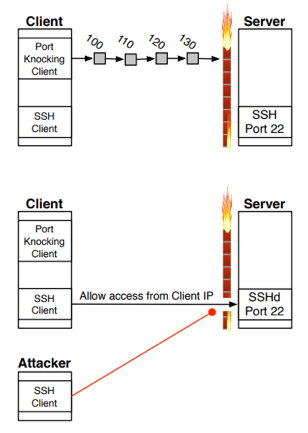
\includegraphics[width=9cm,height=9cm,keepaspectratio]{port_knocking}
\centering
\caption{Port Knocking Replay attack}
\end{figure}

SPA and Port Knocking have the same goal but quite different delivery mechanisms: in this newer system, as the name suggests, all of the necessary information, the so-called "knock", is encoded in a single \textbf{Authorization Packet}.\\
This AP can be sent using TCP, UDP or ICMP, but usually these last ones are preferred.\\
An AP has the following simplified structure:

\begin{itemize}
\setlength{\itemindent}{+4mm}
\item[$\bullet$] \texttt{Timestamp}:1523357581
\item[$\bullet$] \texttt{Client IP}: 2.225.190.3
\item[$\bullet$] \texttt{Password}: somethingsecure
\end{itemize}

Then, what is actually sent to the server is a resulting MD5 hash calculated in this way:
$$ \texttt{MD5(\$timestamp:\$client IP:\$password) = 35b45e73c99905b675ffb05b78714eb9} $$

Once the server received the packet, a SPA daemon will recalculate the hash starting from the password, which must be known from both the client and server, the IP address of the client and the current timestamp.\\
If the resulting hash matches the received one, then the firewall allows that specific client IP to connect to the desired port, otherwise no action is performed.\\
So, we have some advantages using SPA:

\begin{itemize}
\setlength{\itemindent}{+4mm}
\item[$\bullet$] we do not have to respect a certain packet delivery order.\\
It does not seem to be such a big problem, but it is not so unlikely to make it wrong since the server does not send any acknowledge packet back while receiving knock
\item[$\bullet$] the timestamp and client IP within the AP prevent replay attacks
\item[$\bullet$] the use of the password increases security, but clearly there must exists a way to share it with authorized clients
\item[$\bullet$] encoding the packet using MD5 makes almost impossible for attackers to sniff the secret password
\end{itemize}

All these precautions make attackers' life very hard.\\

Coming back to MQTT, we said that username and password could be replaced with an SPA.\\
Applying what we have just discussed to MQTT security, we may think to hide devices, so that they cannot be seen by attackers, and let them communicate just with pre-established brokers.\\
On the other side, we will let brokers communicate only with clients who sent a valid Authorization Packet.\\
More in details: we could have a broker invisible to everyone except for those clients who know the password and send a proper AP.\\\\
\underline{Important}: to make it more secure, we may think to give the broker a list of authorized IP addresses, and reject the communication with any IP not contained in this list, even if able to send a proper AP.\\
Clearly,the bad aspect of this restriction is that it is less scalable.\\

Once a (valid) client have sent a proper AP, the server hosting the broker will allow it to connect to the MQTT dedicated port, and finally the broker will received messages from it.\\
The MQTT port will remain open for a certain (little) period of time, after which the client will have to send another AP to get authorization.\\

We notice that this system is robust even without TLS, and this might be the proper choice to authenticate devices unable to employ encryption, but the problem persists after the authentication: it is true that only messages coming from trusted clients are received by the broker, but if no encryption is used, the messages following the authentication are still vulnerable to MITM attacks.\\

Let's analyze some possible alternative solutions to TLS to face this problem, but keeping in mind that are not totally safe, and \textbf{they should be considered only if TLS is absolutely impossible to use}.

\begin{itemize}
\setlength{\itemindent}{+4mm}
\item[$\bullet$] since authorized users already know the secret password, using it as cipher key and encrypt communication seems to be an almost good idea. We said "almost" for a reason: using the AP password also as cipher key might be dangerous because if an attacker is able, somehow, to discover it thanks to some intercepted messages, then it will also get access granted to the server.\\
Of course, if we assume that the server rejects invalid IP addresses, the attacker will have also to properly spoof its IP.\\
Cracking the password of some intercepted messages is not easy at all, but it is better to be as safe as possible.
\item[$\bullet$] an alternative way might be sending a cipher key to the user once he has successfully authenticated to the server, encrypting the message using the password as a key. In order to guarantee more security, it would be better to generate a different cipher key for each client ip instead of a shared one. Why?
Let's assume that an attacker wants to sniff some messages with the hope of cracking their cipher key: if every client uses the same cipher key the attacker will have a quite bigger number of samples to work with.\\
Besides, using individul cipher keys provides secrecy and integrity: if each client has its own cipher key, then when the server receives an encrypted message from a specific client IP, it tries to decrypt it using the corresponding key and if it succeds it is secure to know who is talking to.\\
We cannot say the same if every client has the same key because if an attacker can crack the messages of even just one client, then he will discover the key used by everyone and, using IP spoofing techniques, he will be able to pretend to be any client.\\

The bad aspect of this solution is that the server would have to keep a, potentially huge, list of client IPs and assigned cipher keys, continuously updated.\\
\end{itemize}

As already said, any of these strategies is safe as a real SDP, which expects the integration of TLS.\\\\

In the next section, let's wrap up the best practices to build a secure MQTT system we have seen so far.\\

\section{Best practices}
\bigskip
Combining all the things we have discussed so far, we can try to list some best practices to consult before creating a very secure MQTT system.
\bigskip
\begin{itemize}
\setlength{\itemindent}{+4mm}
\item[$\bullet$] hiding devices and limiting access to resources/services using SPA with a secure enough password (in this case, secure enough means not vulnerable to brute force and dictionary attacks: attackers must not be able to get accepted from the server trying a huge number of passwords generated or taken by a list)
\item[$\bullet$] efine properly who can communicate with whom: specifically, servers hosting brokers must accept only connections from clients able to send a proper AP (as already said, if our goal is to have a very strong system, the server can keep a list of accepted client IPs, and immediately truncate connections from unregistered ones, even if valid APs are sent); the same is true for clients, so each client must have a list of servers with which is allowed to communicate.
\item[$\bullet$] define an authentication password to specify within the APs, and how to share it with registered clients at the beginning
\item[$\bullet$] define properly the authorizations to assign to clients, such that once a server accepted a client connection, this last one must have access only to authorized resources, that are brokers, specific topics and, even deeper, actions allowed on these ones (publish, subscribe, LWT, retained messages).
\item[$\bullet$] force the client to a further authentication mechanism, that is using credentials to login to a broker. This step is optional, since the client has already authenticated on the server sending the AP, and it seems to be a bit redundant but it might be an additional option.
\item[$\bullet$] encrypting communication using TLS.\\
Standard TLS is already secure enough, but only proves the identity of the server to the client using a X.509 certificate, while the authentication of the client to the server is left to the application layer.\\
To strengthen even more this mechanism, we may think to use mutual authentication, so, as already discussed, the client will send its own X.509 certificate to the server to prove its identity.\\
Then, even the server will be sure that it is talking to a specific, as well as trusted, client.\\
Besides, we have already said that it would be possible to avoid application layer's authentication using client certificates, and this is a feature to consider in order to improve performances.

\item[$\bullet$] thinking about a good load balancing: a large MQTT system may distribute the traffic to multiple MQTT brokers rather than just one, to avoid work overloads.\\
There are many tools to automatize this mechanism, called load balancers and most of them are also able to detect unusually high traffic and block it.
\item[$\bullet$] using tools to detect brute force/dictionary attacks and lock out attackers.
\item[$\bullet$] choose the proper QoS level according to your needs.\\
\end{itemize}

In the next section, we will try to apply in practice the theoritical concepts seen so far, developing an homemade secure MQTT system.\\

\section{Pratical example of building of a secure MQTT system}
\bigskip
This example can be seen as a kind of pratical guide of how to build a \textbf{simplified} homemade, but secure, MQTT system.\\
Before starting, let's see a list of the technologies we are going to use:
\bigskip
\begin{itemize}
\setlength{\itemindent}{+4mm}
\item[$\bullet$] OS: Ubuntu 16.04 Desktop
\item[$\bullet$] Programming languages: Python, NodeJS, Bash
\item[$\bullet$] Redis, Iptables, openssl, Nmap\\
\end{itemize}

By using this minimal set of technologies, we are able to build a quite secure MQTT system. In details, our goals are:\bigskip

\begin{itemize}
\setlength{\itemindent}{+4mm}
\item[$\bullet$] creating a simple MQTT broker
\item[$\bullet$] making server's resorces/services hidden to everyone and accessible only by registered, authenticated and authorized client IPs, by using SPA strategy we have discussed before
\item[$\bullet$] implementing a bruteforce/dictionary attacks detector, able to block attackers
\item[$\bullet$] implementing mutual authentication exploiting X.509 client certificates
\item[$\bullet$] making clients talk only with the server
\item[$\bullet$] sending MQTT messages encrypted through TLS
\item[$\bullet$] looking at an example of publish/subscribe specifying the desired QoS level and retained messages
\end{itemize}

Clearly, \textbf{this is just a simplified demo}, therefore we will make some assumptions along the way.\\

Let's start understanding how to hide resources.

\subsection{Hiding resources}
\bigskip
The first step for the server to avoid connections from/to undesired client IPs is to properly configure its firewall, adding the correct constraint rules.\\
Assuming our tiny system is composed by the following actors:
\bigskip
\begin{itemize}
\setlength{\itemindent}{+4mm}
\item[$\bullet$] Server (\emph{192.168.1.126})
\item[$\bullet$] Client 1 (\emph{192.168.1.6})\\
\end{itemize}

Let's start creating a simple text file containing the list of registered client IPs; let's call it \texttt{"trusted\_client\_ips.txt"}.\\
Then, we move on blocking all the incoming and outgoing connections, except for the ones from/to the registered client IPs on the SPA dedicated port.\\\\
To do that, we simply wrote two bash scripts to properly configure the server and clients' firewall using nothing more than iptables.

\clearpage
\begin{center}
  \lstset{%
    caption=Server's firewall configuration script,
    basicstyle=\ttfamily\small\bfseries,
    frame=tb
  }
\begin{lstlisting}[language=bash]
#!/bin/sh
iptables -P INPUT DROP
iptables -P OUTPUT DROP
file="trsuted_client_ips.lst"

while IFS= read line
do
   iptables -A INPUT -s $line -p tcp --dport 62015 -j ACCEPT
   iptables -t filter -A OUTPUT -d $line -p tcp -j ACCEPT

done < "$file"

iptables -nL

\end{lstlisting}
\end{center}

The above code shows the bash script used to configure the server's firewall; the client's script is almost identical, but \textit{OUTPUT} becomes \textit{INPUT} and viceversa, finally the filename changes to \textit{"trusted\_servers.lst"}.\\


The dedicated port is the only open port on the server, running the Python daemon responsible to accept only registered IPs messages and verify if they are valid APs.\\
\underline{Note}:  an attacker might try to perform brute force or dictionary attacks against this daemon, so we will explain later how to easily protect our system from them.\\

\subsection{SPA mechanism implementation}
\bigskip

The SPA daemon is a simple Python script which accepts secure connections only from the registered client, whose certificate is in server's hands for the following reason: in this demo our server uses the client's certificate as certification authority since it is a self-signed certificate generated locally, but \textbf{in a real scenario we have to rely only on trusted certification authorities, so this is absolutely forbidden}.\\
To make it clear, this is the portion of code where we are going to add the SSL layer:\\

\begin{python}
client, client_address = server_socket.accept()
ssl_version = ssl.PROTOCOL_TLSv1_2

secure_sock = ssl.wrap_socket(client, server_side=True,ca_certs="client.pem",
                               certfile="server.pem",
                               keyfile="server.key",
                               cert_reqs=ssl.CERT_REQUIRED,
                               ssl_version=ssl_version)
\end{python}

\bigskip
Clearly, in order to use these certificates, we first have to create them: it is possible to create self-signed X.509 certificates using the Linux command \textbf{"openssl"}.\\\\
Once the daemon receives an AP (let's notice that messages can come only from clients allowed by IPtables), simply use the pre-established password, the IP address of the sender and the current timestamp to generate the expected MD5, then it compares it with the received one, and if they are equal the received AP is to be considered valid.\\
All of this stuff can be done is few lines of code:\\

\begin{python}

service_port=8883
log_filename="SPA_daemon.log"
SPA_passwd="supersecretpassword"

def grantAccessToClient(client_ip):
	cmd1="iptables -I INPUT -s %s -p tcp --dport %s -j ACCEPT" %(client_ip,service_port)
	
	cmd2='echo "iptables -D INPUT -s %s -p tcp --dport %s 
				-j ACCEPT|at now+2 minute;' %(client_ip,service_port)
				
	os.system(cmd1)
	os.system(cmd2)			        												 
				        												 
			       																							  
def checkAP(received_md5,client_ip):
	timestamp = str(time.time())
	timestamp = timestamp[0:timestamp.find('.')] # avoid ms
	str_to_encode="%s:%s:%s" %(timestamp,client_ip,SPA_passwd)
	expected_md5=hashlib.md5(str_to_encode).hexdigest()

	if(expected_md5==received_md5):
		grantAccessToClient(client_ip)
	else:
		log_file.write("[%s] %s - Invalid MD5 received\n"        %(timestamp,client_ip))
		log_file.seek(0)
	
\end{python}
\bigskip

The idea is pretty simple: if the daemon receives a valid AP, it adds an Iptables rule to allow the client to access the service port, otherwise it does nothing.\\
\underline{Note}: since we want the access to the service to be limited in time, we run the command \textbf{"at"} which gives us the opportunity to run a command after a certain period of time (in the example it is 2 minutes, but in a real scenario it should be larger). Another thing we should notice is that we log only the negative cases, and we do this because there is another script which make us of this log file to detect and block bruteforce/dictionary attacks in real-time.\\

This detector implements a very simple but effective detection strategy: when it reads a new line of the daemon's log file, it takes the client IP address and checks if the number of invalid APs received by him in the last \textsc{time\_range} minutes is larger than \textsc{max\_requests}; if so, that client IP is locked out for \textsc{ban\_time} hours, and to do that we simply add an iptables rule again.\\
This last rule will expire automatically using once again the command "at" to delete it from Iptables.\\
Of course, it is important to define properly these constants: let's say, for instance, that we may accept at most 5 invalid APs for IP in the last 30 minutes and ban the user for 6 hours.\\

We skip the analysis of the SPA client because it is nothing but a Python script which send requests to the server's daemon using sockets and ssl.\\

Instead, we can see a proof of how this SPA mechanism works well, using Nmap to scan the service port, which is the 8883, on the server before and after sending a valid AP.

\begin{figure}[H]
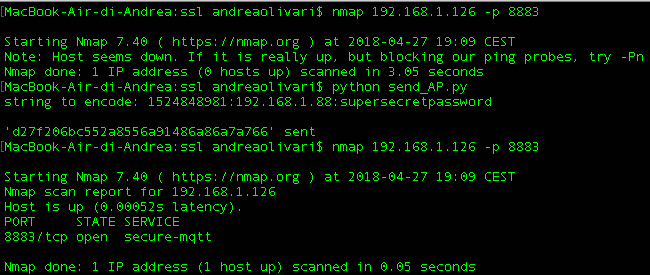
\includegraphics[width=13cm,height=12cm,keepaspectratio]{nmap_proof}
\centering
\caption{Nmap scan before and after sending a valid AP}
\end{figure}

Of course, we had to run a broker on the port 8883, and I have done that using a nodeJS module, called \textbf{Mosca} (\texttt{https://github.com/mcollina/mosca}).\\ Mosca gives the opportunity to use TLS, credentials and two storing methods: MongoDB or Redis.\\
I opted for \textbf{Redis} (\textit{REmote Dictionary Server}), which is  nothing but a key-value store with optional durability, often used to cache server content that needs to be accessed quickly.\\
We skip a deep analysis of the broker's code since it is very similar to the example you can find in the module's page, except for some security constraints we added:

\begin{center}
  \lstset{%
    caption=Mosca broker security settings,
    basicstyle=\ttfamily\small\bfseries,
    frame=tb
  }
\begin{lstlisting}[language=javascript,caption=Mosca broker security settings]
var moscaSettings = {
	port: 8883,
	backend: listener,
	persistence: {
		factory: mosca.persistence.Redis
	},
	secure: {
		keyPath: "../server.key",
		certPath:"../server.pem"
	}
};

var server = new mosca.Server(moscaSettings);

server.on('ready',function() {
	console.log("MQTT broker is up and running");
	server.authenticate = function(client,username,password,callback) {
		callback(null,(username===broker_username && password.toString('ascii')===broker_password))
	}
});
\end{lstlisting}
\end{center}


At this point, MQTT clients can be implemented using Python once again, and more in details its library \textbf{paho.mqtt} (available also in Java and other languages), to simply connect to the broker and publish/subscribe to topics.\\
This library is so easy to use, and allows us to set TLS, credentials, QoS levels and retained messages in no more than one line of code for feature:\\

\begin{python}
def publishMsg(client,topic,message,qos_level,retain_msg):
	print("publish data")
	client.publish(topic,payload=message,qos=qos_level,    					retain=retain_msg)

client = mqtt.Client()
ssl_version = ssl.PROTOCOL_TLSv1_2
client.username_pw_set("brk_username",password="brk_pass")

client.tls_set("../server.pem",cert_reqs=ssl.CERT_REQUIRED,tls_version=ssl_version)
publishMsg(client,topic_pub,"online",1,True)
\end{python}


\chapter{Internship experience}
\section{Introduction}
\bigskip
I did my internship working for 4 months with a company called ABO DATA, which deals with IoT technologies.\\
The company enables customers to customize and manage IoT business applications: most of times we talk about customers' devices/sensors which send their measurements to a cloud or a centralized system, then these measures are computed and exploited to do something else related to customers' business.\\
So, during my internship in the company I often had to deal with tasks related to receiving data from a source and their subsequent forwarding to a destination, like a bridge, and most of times I worked with two protocols: HTTP(s) and MQTT.\\

In the next page, I would like to discuss two real-world cases I have worked on, which should make us reasoning about how a productive system should be thought and implemented.\\

\clearpage
\section{Case 1 - Real-world MQTT-based industrial system}
\bigskip
This is a real-world scenario involving an important company, whose name cannot be disclosed for reasons of privacy, partner of several automotive, pharmaceutical, writing tools and watchmaking industries, that produces and distributes automated systems as well as high-precision and efficient cutting tools.\\

This company recently decided to build a realiable monitoring and management system for their machines using a Cloud architecture.\\
This proposal's goal is to collect data from machines' sensors in order to:

\begin{itemize}
\setlength{\itemindent}{+4mm}
\item[$\bullet$] create a so-called \textit{Local Control Room}, which allows the company's customers to check the performances, real use and health status of their machines, in real-time
\item[$\bullet$] create a so-called \textit{Centralized Control Room}, which allows the company itself to monitor their resources operating on different customers in order to collect historical data useful to make analysis and comparisons
\end{itemize}

These monitoring systems collecting tons of data are often used by companies and industries to drastically change and improve their maintenance approach.

\begin{figure}[H]
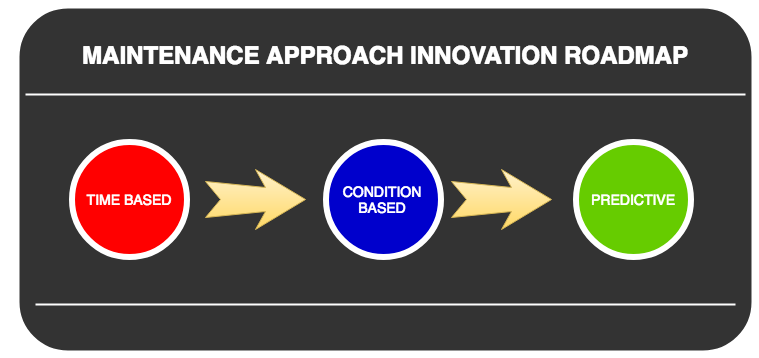
\includegraphics[width=10cm,height=10cm,keepaspectratio]{maintenance_approach}
\centering
\caption{Maintenance approach innovation roadmap}
\end{figure}

A \textbf{Time-based} maintenance approach is the simplest one, and unfortunately the most used, so when a machine breaks down, the customer contacts the company support to receive assistance.\\
The use of a monitoring system introduces a new maintenance approach, called \textbf{Condition-based}, thanks to which the corrective maintenance is considerably reduced; in fact, the continuous monitoring of the health status of the machines allows to intervene before the failure occurs.\\
Finally, in the last few years a new approach, called \textbf{Predictive}, was born; this approach is based on the possibility of predicting possible failures in a smart way, using the huge amount of data received as input for Machine Learning algorithms.\\

Clearly, both the second and third approaches can be seen in two different ways:

\begin{itemize}
\setlength{\itemindent}{+4mm}
\item[$\bullet$] the customer uses data from its Local Control Room, and when he (or his ML algorithms) detects an imminent breakdown, he contacts the company assistance
\item[$\bullet$] the customer uses data from its Local Control Room for other purposes, and let the company predicting possible failures using Centralized Control Room's data.\\
\end{itemize}

Now that we know what a monitoring system can be useful for, let's see the structure of the system mentioned above.\\

This company provides two different monitoring systems for two different possible scenarios:
\bigskip
\begin{enumerate}
\setlength{\itemindent}{+5mm}
\item \emph{Factory}
\item \emph{Connected machines}
\end{enumerate}

\clearpage
\subsection{Factory}

\begin{figure}[H]
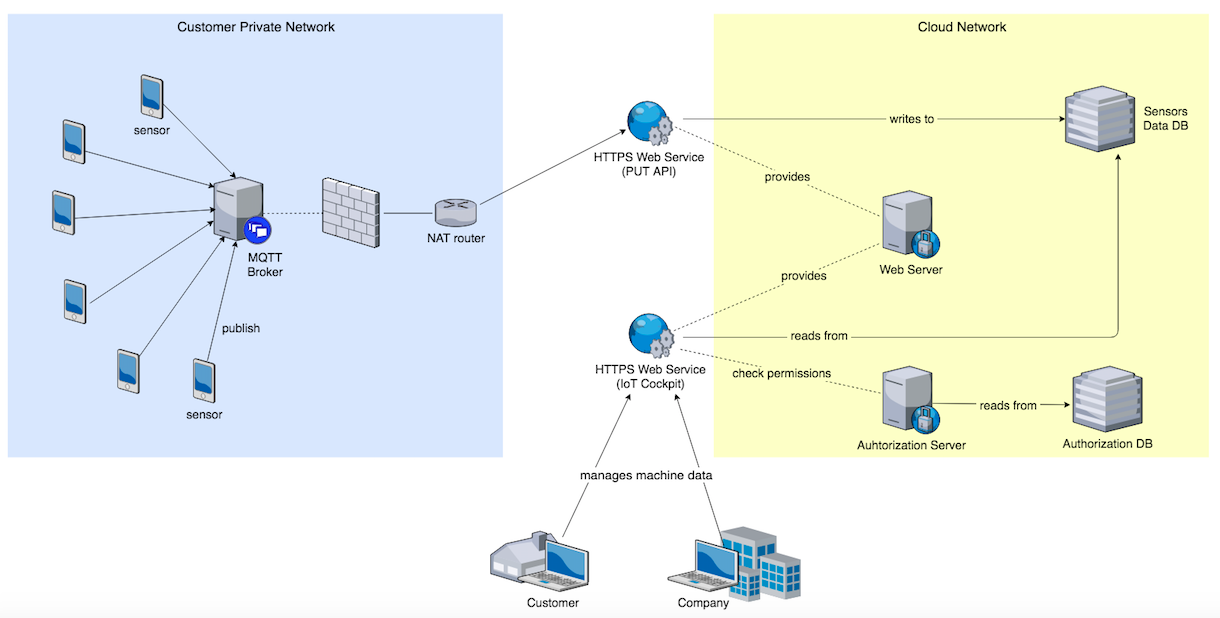
\includegraphics[width=15cm,height=11cm,keepaspectratio]{factory_architecture}
\centering
\caption{Factory Architecture}
\end{figure}

This first scenario expects the customer to be an industry, having its own private network to which the company's machines (equipped with internal sensors) are connected.\\
As we can see in the above image, the customer runs a MQTT broker on a local server to which the company's sensors publish their data.\\

This MQTT broker is developed, provided and properly configured by a third company, which is the owner of the Cloud network as well as the provider of the monitoring service, and in our case we are talking about \emph{SAP}.\\
In this specific scenario, MQTT communication is not encrypted and there is no required authentication system; simply, there are several open topics, one for each sensor, where these last ones publish their measures at regular intervals of time.\\
It is easy to understand that this is a risky choice for an industrial system architecture, that should be considered only if we can totally trust all the devices connected to the internal network.\\
Clearly, to trust all of them we have also to be sure that the internal network protection is secure enough: having a wired network defintely helps, since an attacker must physically access the building to connect its malicious device, but of course this is not always possible, especially when devices belonging to the same network are not located in the same building.\\
In that case it is necessary to create a secure wireless network protected by strong passwords.\\

As shown above, the customer private network increases its security putting a firewall in front of the server hosting the MQTT broker.\\
This firewall is properly configured to hide all the devices from the external world, blocking all the incoming and outgoing connections.\\
Actually, there is only one outgoing connection allowed, that is the one that allows the server, on which the broker runs, to send the data collected by the sensors to the cloud.\\
Before going on, I would like to clarify that putting a firewall in front of the server is a good practice and gives the network a robust protection, but in this case, having a \emph{NAT} router which does not any port forwarding and no mapping between the public IP address and the internal ones, using it seems to be a little redundant.\\

So, we were saying that there is one outgoing connection allowed: this is nothing but the request sent by the local server to transmit sensors' data to the cloud.\\
To do that, it exploits an \emph{HTTPS API} (simply a web service), provided by a webserver belonging to the Cloud network, so to the SAP network, whose job is to receive data from sensors and write them on the database.\\
Having to do with a secure HTTPS connection we know that data is transferred safely, therefore we can assume that the customer-side is properly protected.\\

There is just one remaining risk to be removed: only trusted clients' requests must be accepted by the \emph{PUT API}, hence those coming from the company customers' broker servers.\\
To do that, mutual authentication is required, so when a customer's broker sends sensors' data to the API it will send even its own X.509 certificate to the remote webserver to prove its identity.\\
\underline{Note}: this is the solution chosen and implemented by SAP, but an alternative one could be to include authentication credentials in the POST content, avoiding the mutual authentication mechanism, which, as already seen, can afflict performances.
We will discuss more in detail about this at the end of the next section, related to the Connected Machines architecture.

We should notice that the Factory architecture brings a great benefit in terms of certificates management: since all the customer's machines/sensors belong to the same private network and only the server is allowed to establish outgoing connections, then just one X.509 client certificate is necessary for all of them.\\

One last thing to notice is that, considering what has been said so far, it seems that the customer has no way to verify if the data sent to the API has been correctly received and stored on the Cloud.\\
This is not true, in fact the customer, as well as the company itself, can verify the health status of their machines using another secure web service, called \emph{IoT Cockpit}, provided by the same webserver.\\
This service simply provides an intuitive dashboard to the user, by which he can stay updated and check their machines and measures; the difference from the other API is that this last one requires a user authentication and can be accessed from any network.\\


\subsection{Connected Machines}

\begin{figure}[H]
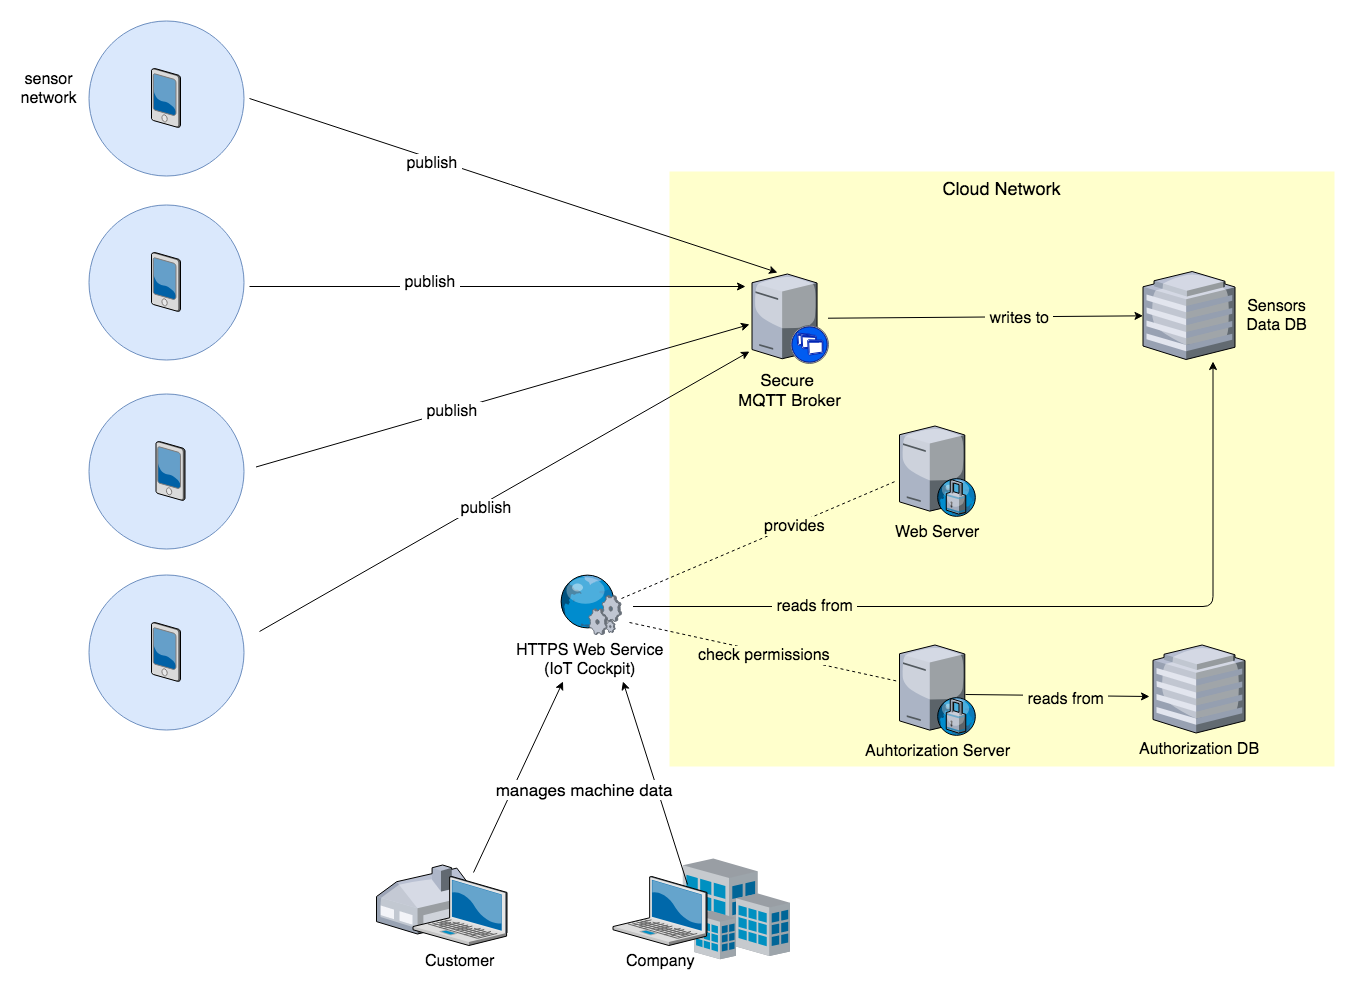
\includegraphics[width=14cm,height=11cm,keepaspectratio]{connectedmachines_architecture}
\centering
\caption{Connected Machines Architecture}
\end{figure}

This second system architecture deals with a different and more difficult to protect scenario.\\
In this case, there are several customers' machines positioned in different places, probably far from each other, therefore no common and secure network protecting them, but simply standalone machines and their related sensors.\\
It is obvious that this fact changes everything: it would not make sense to give each machine a local server running an MQTT broker to which send data, and then forward it to the cloud through it as before.\\
This procedure should be considered only when there are several machines close to each other which can share a private network in order to create a singular exit node towards the cloud network.\\

Having customers' sensors spread all over the world is a very common scenario; just think about sensors applied on transports, for instance sensors used to check the health status of car tires.\\

So, for all these cases there is only one way to communicate: have a remote MQTT broker on the cloud and let each sensor publishes its own data on it.\\
Clearly, this time it is necessary to use the secure version of MQTT, therefore relying on TLS.\\
As before, it is also necessary to verify if sensors' data actually come from trusted senders, so mutual authentication is required again.\\

Now that we have seen that mutual authentication is used in both the architectures, I would like to briefly discuss this implementative choice: previously, I told you that using mutual authentication could be replaced by authentication credentials sent along with POST data in order to spare computational time; in this last architecture it would be necessary to create credentials for each individual sensor, but we know that the number of sensors can be huge and this can be a little inconvenient.\\
Unless you use access tokens, using login credentials and sending them at every request would be extremely heavy for the server that should verify them, browsing a very large database continuously; this would result in a perceptible slowdown in the application layer and a large memory consumption.\\
To achieve better performances, someone may think to use the same credentials for multiple sensors, or even all of them, in order to avoid having to deal with a huge number of records, but this would be a risky choice because if the credentials of a sensor are stolen, then many will pay the consequences.\\
Using client certificates, this problem does not exist, in fact if the private key of a sensor's certificate is stolen, only that specific sensor will be in trouble.\\
As we have already seen, another benefit of using client certificates is that authentication is moved from the application layer to the transport one.\\

Here we have a practical example of what we discussed before in the section dedicated to the construction of an homemade MQTT system: I recommended you to trust only certificates approved by reliable certification authorities and never trust self-signed certificates. \\
In the homemade demo, our server trusts the client's self-signed certificate because it stores it locally, but this last architecture helps us to understand that, in addition to the fact that it is not good to trust self-signed certificates, forcing the server to keep a potentially huge number of certificates is not convenient and totally pointless; therefore, the right way is to trust client's certificates which are trusted by certification authorities we trust.\\

\bigskip

After having seen these two real-world architectures, we can conclude that there is no single perfect solution covering all cases, but it is necessary to find the most proper one for the specific case we are dealing with, considering all the relevant factors, such as networks topologies, performances, secrecy, integrity, users' needs, maintenance.\\



\section{Case 2 - Every aspect is important }
\bigskip
This second case is certainly less detailed than the previous one, but I would like to quickly discuss it because it helps to show how every aspect of a system should be considered important as the others, and as trivial errors can lead to serious consequences.\\

In the previous case we have seen that the monitoring system was provided by SAP; we can say that, currently, the company relies on the SAP platform for most of its projects, and SAP structure is very solid and secure, paying attention to remain updated with the newest security measures to take.\\
For more information, you can consult their official documentation at \\ \texttt{https://www.sap.com/corporate/en/company/security.html}.\\

This is a real case, but, for obvious reasons of privacy again, I will not be able to give a name to the customer I am going to talk about.\\

I worked on a project where I had to take some real-time data stored on a remote server belonging to the customer and send them to another remote server through a secure MQTT channel.\\
I started Wireshark to sniff data and see if it was possible for an attacker to alter the measures, but without success as the MQTT channel used TLS.\\

What we did not say is that the protocol used to recover data from the source server was FTP, which is known to be extremely vulnerable since it sends data in plain-text.\\


So, the moral of this brief story is that it is fundamental to consider every security aspect of the system before developing it, because all the efforts involved in the successful implementation of a communication channel can be undermined by a very bad implementation of another communication channel.\\


\part{ZigBee}

\chapter{Protocol Overview}

\section{Introduction}
\bigskip

We have already seen in the MQTT part that nowdays there are a lot of high data rate communication involving very constrained devices.\\
For this reason, we need some standard providing low-latency with low-energy consumption even at lower bandwidths.\\

More in details, these are the requirements for a network full of constrained devices:

\begin{itemize}
\setlength{\itemindent}{+4mm}
\item[$\bullet$] be able to scale to larger sizes and operate for years without manual intervention
\item[$\bullet$] extremely long battery life for devices
\item[$\bullet$] granting a good quality of services
\item[$\bullet$] low complexity and low cost communication
\end{itemize}


In the previous part we have discussed MQTT, which is very different from ZigBee, in the way it works and in the real world usages.\\

ZigBee is a low-cost emerging protocol deployed by ZigBee Alliance, for controlling and monitoring applications, covering 10-100 meters within the range. \\
This communication system is less expensive and simpler than Bluetooth and Wi-Fi and its range can be extended using routers, as we will see in a minute.\\

Nowadays, ZigBee is mainly used in the following fields of application:
\begin{itemize}
\setlength{\itemindent}{+4mm}
\item[$\bullet$] \textbf{Industrial automation}: industries exploit ZigBee to manage and continuously monitor critical equipments.\\
Why ZigBee and not simply Wi-Fi or Bluetooth? Because it has lower communication costs than Wi-Fi and a higher communication range than Bluetooth, hence it optimizes the control process.
\item[$\bullet$] \textbf{Smart Home}: this protocol is perfectly suited for controlling home appliances remotely. We may think to TVs, surveillance devices, locks, thermostats, lighting system, garage door, windows, blinds, speakers, as well as any other home system that can be controlled remotely.\\
Currently, this is the most common ZigBee application.\\

\end{itemize}

In the next section let's start to analyze the architecture and the basic concepts of this protocol.\\

\section{Architecture and basic concepts}
\bigskip

\begin{figure}[H]
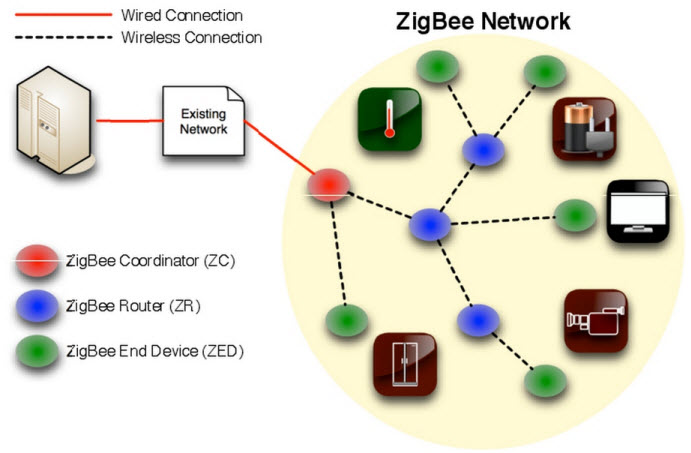
\includegraphics[width=12cm,height=12cm,keepaspectratio]{zigbee_architecture}
\centering
\caption{ZigBee Architecture}
\end{figure}

\bigskip
\subsection{ZigBee components}
\bigskip

As we can see in the above picture, the ZigBee system consists of three types of devices:

\begin{itemize}
\setlength{\itemindent}{+4mm}
\item[$\bullet$] \textbf{Coordinators}: they manage the overall network and they are responsible for starting it, allowing other devices to join it, keeping trace of them, handling and storing the information while performing transmission data operations, configuring the security level of the network.\\
A coordinator is considered as the \textbf{Trust Center (TC)}, which performs security control of the network, stores and distributes the network keys.\\
For all these reasons, the coordinator never sleep, instead it must be continuously powered.


\item[$\bullet$] \textbf{Routers}: they are intermiediary devices responsible for routing packets between end devices or between an end device and the coordinator.\\
Routers, as well as end devices, need to be accepted in the network by the coordinator.\\
Routers have two things in common with the coordinator: 1) they cannot sleep, 2) they can give permissions to new devices to join the network.

\item[$\bullet$] \textbf{End devices}: they are low-power, or battery-power, devices (usually sensors) that can communicate only through their parent nodes (we will explain this better in a few pages).\\
Unlike routers, end devices cannot route traffic and they can go to sleep to reduce power consumption.
\end{itemize}

There is no required number of specific components for a ZigBee network, instead the number of coordinators, routers and devices depends on the network we want to build and its topology (\textit{star, cluster tree or mesh}).

\subsection{ZigBee network topologies}

\begin{figure}[H]
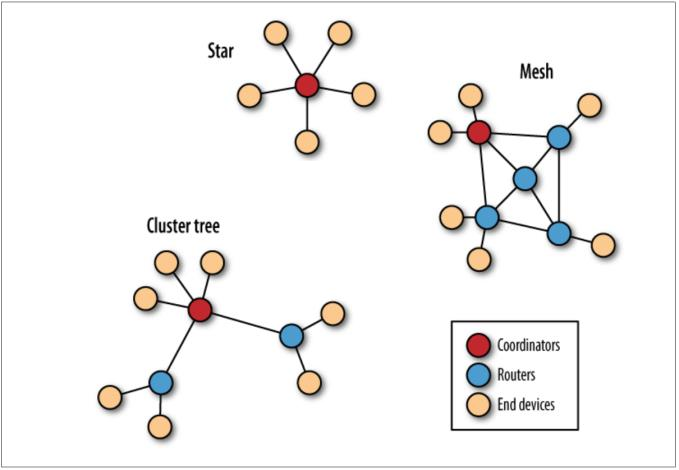
\includegraphics[width=11cm,height=11cm,keepaspectratio]{zigbee_topologies}
\centering
\caption{ZigBee Topologies}
\end{figure}

\begin{itemize}
\setlength{\itemindent}{+4mm}
\item[$\bullet$] \textbf{Star}: in this topology there is only the coordinator responsible for initiating and managing the network devices; since every device talks directly with the coordinator, we consider the other devices as end devices, therefore no routers in this topology.\\
This topology is mainly used when all the endpoints need to communicate with a central controller, so likely in industries.\\
Of course this topology is very simple, but its simplicity is also its greatest weakness, in fact the coordinator is a single point of failure, because if it breaks down the whole network goes down.

\item[$\bullet$] \textbf{Tree}: this topology has a root node, represented by the coordinator, which is responsible for establishing the network and choosing the proper key network parameters.\\
This time we have even routers, which can have either the coordinator or another router as parent node, and they are responsible for routing data packets through the network using hierarchical routing strategy.\\
This solution is not so better than the previous one because we still have a single point of failure, given by the coordinator, besides children nodes become unreachable if their parent node breaks down.

\item[$\bullet$] \textbf{Mesh}: this topology has, as usual, a single coordinator, several routers to extend the network and, of course, end devices.\\
Once again, the coordinator establish the network and is responsible to choose key network parameters.\\
As before, there is no more a single point of failure, besides in this case we have multiple paths to reach a node, therefore a more robust protection from link failure.\\
The only drawback of this topology is that is complex and more difficult to setup than the previous ones.\\
\end{itemize}

Mesh topologies are more robust than cluster the other two, therefore they are the most used.\\

\clearpage
\subsection{Protocol Stack}
\bigskip

The protocol is based on the IEEE 802.15.4 standard, which provides the physical and MAC layers, while the above layers we are going to see are given by ZigBee.
As usual, each layer provides a set of services exposed to the upper layer.\\

\begin{figure}[H]
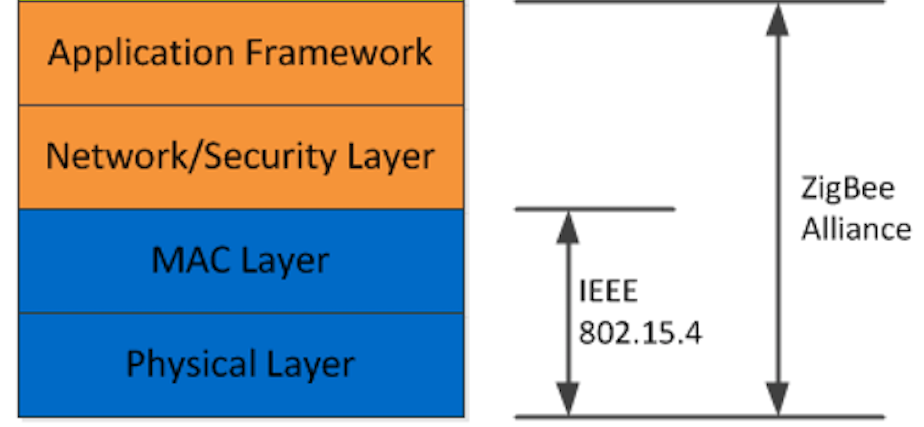
\includegraphics[width=8cm,height=10cm,keepaspectratio]{zigbee_protocol_stack}
\centering
\caption{ZigBee Protocol Stack}
\end{figure}

More in details, let's briefly see them: 

\begin{itemize}
\setlength{\itemindent}{+4mm}
\item[$\bullet$] \textbf{Physical Layer}: this layer, as the next one, is provided by \emph{IEEE 802.15.4} standard, and defines the physical features and operations of ZigBee devices, such as power, channels, modulation, demodulation, transmission rate, etc.
\item[$\bullet$] \textbf{Medium Access Control layer (MAC)}: it manages data transmissions among devices. For instance, it provides services like transmission retry and acknowledgment management.
\item[$\bullet$] \textbf{Network Layer}: it is responsible for securely transmit frames through the network. 
About frames, it is important to say that ZigBee exploits a frame counter in order to ignore duplicate messages and stop possible replay attacks.\\Besides, transmitted frames are protected using cryptographic algorithms, such as AES for secrecy, ensuring its integrity using a \emph{Message Authentication Code (MAC)}.

\item[$\bullet$] \textbf{Application Layer}: it consists of ZigBee device objects (ZDOs), Application support sub-layer (APS) and the Application Framework, where: 

\begin{itemize}
\item \emph{ZDOs} are applications supporting layer primitives used by end devices, routers and coordinators.\\ 
Furthermore, ZDOs manages the security policies and configuration of a device.
\item \emph{APS} provides a communication bridge between the Network Layer and the Application Layer, collaborating with the network layer to establish and managing cryptographic keys, and provides primitives for the management of cryptographic keys to the upper layers.
\item \emph{Application Framework} is nothing but the environment in which application objects are hosted.\\

\end{itemize}
\end{itemize}

\subsection{ZigBee communication modes}
\bigskip
ZigBee employs two communication ways:
\bigskip
\begin{itemize}
\setlength{\itemindent}{+4mm}
\item[$\bullet$] \textbf{Beacon} mode: the coordinator sends a beacon message periodically to the devices and these last ones wait for it before sending messages addressed to the coordinator.\\
When the transmission is completed, the coordinator set a schedule for the next beacon so that the device goes to sleep till that moment.\\
In some cases, even the coordinator can go to sleep mode.\\
Beacon intervals can be from 15 ms up to 252 seconds.\\
So, in this mode, all the devices know when to communicate with each other.\\
Beacon mode is mainly used when the coordinator runs on batteries, hence it needs to save as much power as possible.

\begin{figure}[H]
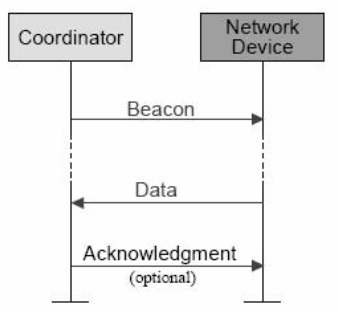
\includegraphics[width=6cm,height=6cm,keepaspectratio]{zigbee_beaconmode}
\centering
\caption{Beacon mode}
\end{figure}

\item[$\bullet$] \textbf{Non-Beacon} mode: in this case the coordinator is mains-powered and wait continuously for data from the devices, which can transmit at random intervals.\\
This mode is used in systems where devices are almost always 'asleep' (for instance, in smoke detector systems).\\
Clearly, it might happen that an end device finds the channel busy and in that case the coordinator will miss the call.

\begin{figure}[H]
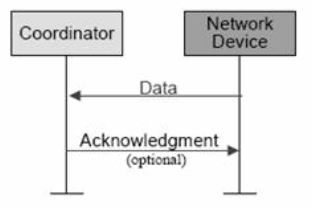
\includegraphics[width=6cm,height=6cm,keepaspectratio]{zigbee_nonbeaconmode}
\centering
\caption{Non-Beacon mode}
\end{figure}

\end{itemize}

In the next chapter, we are going to discuss the security aspects of this protocol.\\

\chapter{Security Overview}

\section{Introduction}
\bigskip
As already said in the MQTT part, IoT will play a primary role in the coming years and for this reason it is fundamental to take care about its security.\\
While MQTT security is mainly aimed to help companies and industries to transfer their production data reliably, ZigBee has more to do with personal area networks that interconnect devices primarily for personal uses, hence high personalized and sensitive data.\\
Just think to a smart home based on ZigBee: a lot of user sensitive information can be leaked by an attacker if the security aspect is neglected.\\
Data theft is not the only problem, in fact an attacker would cause a lot of problems to the user if he could control his household appliances.\\
Just think about a thief, good enough to find and exploit a ZigBee vulnerability and turn off the surveillance devices.\\\\

In the next chapters, we are going to discuss the security measures offered and adopted by the ZigBee standard; more in details, we will analyze its security models, keys (types, generation and management), authentication mechanisms and protection from some famous attacks.\\


\clearpage
\section{Security assumptions}
\bigskip
Being ZigBee a simple as well as low-cost communication protocol, it relies on a symmetric-key cryptography to protect network messages and devices, precisely AES 128 bits, avoiding heavier encryption system, like the asymmetric one; therefore, both originator and recipient of a protected transaction need to share the same key.\\
All the ZigBee security features we are going to discuss are strictly related to the cryptographic (symmetric) keys used by the protocol; in order to talk about them, we must first take a look at the following list of assumptions on which they are based:

\begin{itemize}
\setlength{\itemindent}{+4mm}
\item[$\bullet$] \emph{ZigBee employes an open-trust model}, which means that the stack layers trust each other, therefore the layer that originates a frame must secure it
\item[$\bullet$] \emph{communication between different stack layers on the same devices is not encrypted}
\item[$\bullet$] \emph{cryptographic keys are securely stored in quite-resistant hardware devices}
\item[$\bullet$] \emph{keys are always transmitted encrypted}, so never revealed
\item[$\bullet$] \emph{cryptographic mechanism and security policies are properly implemented}
\item[$\bullet$] \emph{Availability of almost perfect random number generators}\\
\end{itemize}

\clearpage
\section{Security models}
\bigskip

ZigBee provides two network security architectures, or models: \emph{distributed} and \emph{centralized}.\\

\begin{figure}[H]
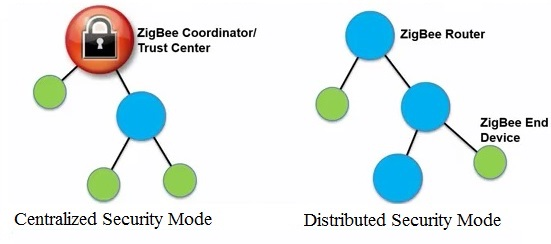
\includegraphics[width=10cm,height=10cm,keepaspectratio]{security_models}
\centering
\caption{ZigBee Security Models}
\end{figure}

The difference between them concerns only the way they accept new joining devices into the network and how messages are protected.\\

The idea of the \emph{distributed security model} is pretty simple: there is no coordinator, but only routers and end devices.\\
In this model, we totally rely on routers to accept new routers and end devices within the network as well as to generate and distribute network keys.\\
We will talk better about this in the next chapter, but just to understand what we are going to say we should know that each network has a key used to encrypt broadcast messages, called \emph{network key}, and a key shared by two devices to communicate, as well as to encrypt and provide the network key, called \emph{link key}.\\
This security model expects all the devices to share the same network key and to be pre-configured with the same link key.\\

The \emph{centralized security model} is a bit more complex, but even more secure.\\
In this case we have routers, end devices and the coordinator, that from now on we will call \emph{Trust Center (TC)}.\\
This time the responsible for the management and acceptance of routers and end devices joining the network as well as the creation and sharing of the keys is the TC.\\
Besides, it will also create and provide a new network key periodically, in order to protect the network from possible attackers, who can try to stole it.\\

So, The first model is certainly simpler but even less secure, and almost not used, so we will focus more on the second one}.\\

\section{Security keys types and management}
\bigskip
We have already mentioned that a ZigBee network exploits two main types of keys to communicate safely: \textbf{network keys} and \textbf{link keys}. Actually, there is also a third key, called master key.\\
Let's see them in details:

\begin{itemize}
\setlength{\itemindent}{+4mm}
\item[$\bullet$] the \emph{network key} is a 128-bit key generated and distributed by the Trust Center to all the network devices in order to allow them to communicate in broadcast securely.\\
It is clear that the TC cannot send the network key in plain-text, otherwise an attacker could sniff that, making it useless.\\
There are two types of network keys, \emph{standard} and \emph{high security}, which differ from each other in the way they are distributed to joining devices. More specifically, a high-security network key is sent encrypted, the other one in plain-text.\\
It is important to notice that joining devices can be also pre-configured with a network key, but this is a uncommon practice, since, as already said,  in a centralized model the network key is updated periodically by the TC.
\item[$\bullet$] the \emph{link key} is a 128-bit key shared by two devices, so between the TC and another node, or between two nodes.\\
More in details, we have four different types of link key:

\begin{itemize}
\item \emph{Pre-configured Global Link key}: it exists only for one reason, that is encrypting the network key in order to transfer it safely from the TC to the devices.\\
As the words \emph{global} and \emph{pre-configured} suggest, this key is the same for all the network nodes and usually pre-installed in the devices that want to join the network.
\item \emph{Pre-configured Unique Link key}: same use of the previous one, but different for every node.
Let's clarify that pre-configured keys are usually defined by the manufacturer of the device, or simply by ZigBee.
\item \emph{Install Code}: it is nothing but another pre-configured link key based on the assumption that every ZigBee device can have a unique 128-bit install code.\\
We can instruct the TC to require to every new device to use its own install code to join the network; clearly, we have to previously store the code within the Trust Center in order to check if it matches the one provided by the device.
\item \emph{Trust Center Link Key (TCLK)}: like the last one, this key is used to allow the TC and another node to communicate securely, but the difference is that this time it is not pre-configured.\\
Clearly, we need an algorithm to obtain it: it is possible to simply make the TC generating it randomly or derive it from the pre-configured unique link-key using the  the Matyas-Meyer-Oseas hash function.\\ 
Without entering in too many details about this hash function, we should say that it takes two 128-bit keys as input and return one 128-bit key as output; the second input key of the function is known only by the TC.\\
Of course, this generated key must be sent to the interested node, and to do that the TC exploits once again the network key or, much better, the pre-configured unique link key, if existent.\\
A reasonable question is \emph{"why should we generate a TCLK if we already have a pre-configured link key?"}; I did not find a specific answer to this question, but I guess that the reason is that, being the pre-configured link key rarely updated, changing the link key we use to communicate and avoiding to use our pre-configured link key helps us to simply protect it and give less chance to an attacker to be able to stole it.
\item \emph{Application Link Key}: similar to the previous one, but used by a pair of nodes.\\
The generation and provisioning of the key is quite intuitive: one of the two devices requests the key to the TC, which is responsible to generate and send it to both of them using their respective pre-configured unique link key or, if not existent, the network key.
\end{itemize}

\item[$\bullet$] the \emph{master key}: is a key from which link keys can be established by two devices, without having to communicate with each other. Clearly, both the devices must have the master key.

\end{itemize}

Now that we have analyzed the ZigBee security keys and their provisioning ways, I would like to report, just for completeness, that there exists an extension of the traditional key-transport, which involves certificates.\\
Security keys can be distributed using the \emph{Certificate-Based Key Establishment protocol (CBKE)}, which implements a mechanism to allow devices to negotiate symmetric unique keys with the TC, starting from a certificate, signed by a Certification Authority, that both devices must have. So, every device in the network is expected to store a certificate signed by a trusted certification authority.\\
The CBKE mechanism allows the device to start communicating, but even the Trust Center to safely identify it and prevent unauthorized devices to join the network.\\
The key establishment procedure involves the following four steps:

\begin{enumerate}
\setlength{\itemindent}{+5mm}
\item Exchange static data for certificate validation
\item Generate the key
\item Derive a MAC (\emph{Message Authentication Code}) key
\item Confirm the key using the MAC
 \end{enumerate}

Just for completeness, we have to say that the key generation and the MAC derivation exploit two mathematical functions which are, respectively, the Elliptic Curve MQV and a Key derivation function, but we will not delve into them as they go beyond the context.\\
At the end of this process, both the Trust Center and the device \emph{i} share a new Link Key LK\textsubscript{i}, which is used to encrypt the TCLK they are going to use to communicate.\\
Now, if two devices \emph{i} and \emph{j} have obtained their TC Link Key, and want to communicate with each other, they can obtain their Application Link key by asking it to the Trust Center, as usual, which will generate a random Application Link Key LK\textsubscript{ij} and send it to both the devices using their respective Trust Center Link Key.\\

\subsection{Over-The-Air Updates}
\bigskip
We have already mentioned that in a centralized architecture the TC periodically updates and distributes the network key in order to not give attackers much time to try to acquire it.\\
Clearly, the updates of the network key are sent over-the-air, so they must be encrypted with some keys, which usually are either the current network key or the Trust Center Link key (unique or global, depending on the individual node).\\
Obviously, the second one is a better and safer choice, because if an attacker has already stolen the current network key, and the Trust Center uses such key to encrypt the new one, then the attacker will always be able to get the updated network key.\\
Let's clarify that each node is able to store several network keys, but also to identify the current one with a unique key sequence number assigned by the Trust Center.\\

Keys are not the only things we may think to update over the air, in fact ZigBee gives the user the chance to update a device, adding new features as well as applying security patches, if necessary.\\
Clearly, if this kind of communication is not protected enough, it might happen that devices accept some critical fake updates from untrusted sources.\\
Assuming, for instance, we want to send an updated code image to a device to apply a security patch, we firstly sign the image with a private key k\textsubscript{1}, then we send the image over the network using a second cipher key k\textsubscript{2}; doing this way only the end device will be able to decrypt it and verify the validity of the image thanks to its signature (it is clear that the end device must know the two keys used to encrypt and sign).\\
Once the device received the message, it decrypts and validates it, then updates itself.\\

\clearpage
\section{Protocol Stack Security}
\bigskip
In this section we are going to discuss the security measures adopted by the ZigBee protocol stack, which involves the MAC, Network and APS layers.\\

The IEEE MAC Layer implements security services which are used by the ZigBee protocol in the network and application layers.\\ 
IEEE 802.15.4 establishes the encryption algorithm to use when the data has to be transmitted, which is AES with a 128-bit key, but the standard does not specify how the keys have to be managed or the authentication policies to be applied.\\
This is a task concerning the upper layers, hence ZigBee is responsible for that.

\subsection{802.15.4 Security}
\bigskip

\subsubsection{Security Control Header}
\bigskip
Let's start taking a look at the structure of a MAC frame before going on.\\

\begin{figure}[H]
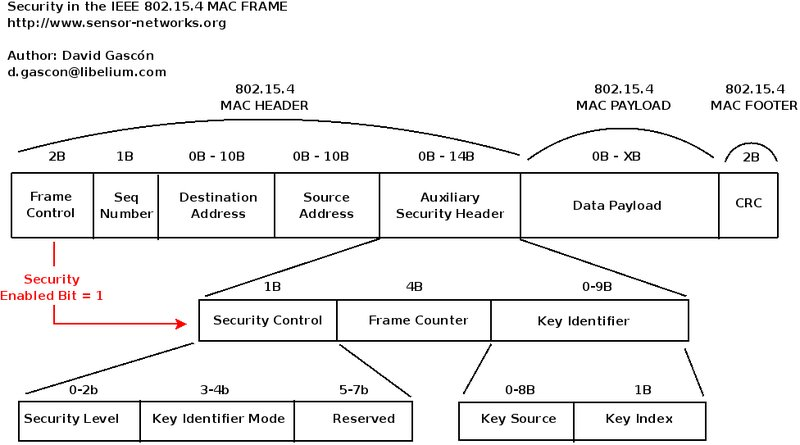
\includegraphics[width=13cm,height=13cm,keepaspectratio]{mac_frame}
\centering
\caption{ZigBee MAC Frame's Structure}
\end{figure}

As we can see in the image above, IEEE 802.15.4 MAC frames contain a specific header dedicated to security, called \emph{Auxiliary Security Header}.\\
Thie header is enabled only if the \emph{Security Enabled} bit, contained in the \emph{Frame Control} field, is set to 1.\\
There are three subfields inside the Auxiliary Security Header:

\begin{itemize}
\setlength{\itemindent}{+4mm}
\item[$\bullet$] \emph{Security Control}: it is used to specify the type of protection provided by the network.\\
The most important subfield of the Security Control field is \emph{Security Level}, which can assume eight different values, each of them providing a different degree of encryption and integrity checks, and is the place where out global security policy is set.

\begin{center}
\small
   \begin{tabular}{ | p{3cm} | l | l | p{3.5cm} |}
    \hline
    Security Level Identifier & Security Attributes & Data Encryption & Data Authenticity Checks \\ \hline
    0x00 & None & N & N \\ \hline
    0x01 & AES-CBC-MAC-32 & N & Y\\ \hline
    0x02 & AES-CBC-MAC-64 & N & Y \\ \hline
    0x03 & AES-CBC-MAC-128 & N & Y\\ \hline
    0x04 & AES-CTR & Y & N\\ \hline
    0x05 & AES-CCM-32 & Y & N\\ \hline
    0x06 & AES-CCM-64 & Y & N\\ \hline
    0x07 & AES-CCM-128 & Y &N\\ \hline
    \end{tabular}
\end{center}
\bigskip
The Data Payload field can have three different configurations, depending on the previously defined security fields:

\begin{figure}[H]
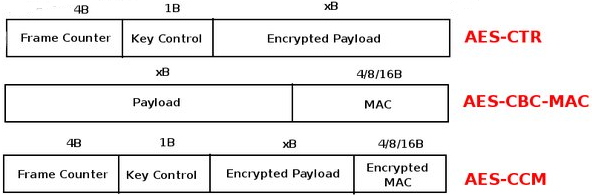
\includegraphics[width=10cm,height=9cm,keepaspectratio]{datapayload_fields}
\centering
\caption{Data Payload possible configurations}
\end{figure}

\begin{itemize}
\setlength{\itemindent}{+4mm}
\item \emph{AES-CTR}: we encrypt data using the AES algorithm combined with a 128-bit key.
\item \emph{AES-CBC-MAC}: payload data is not encrypted, but a Message Authentication Code (MAC) is computed and attached to the end of the data payload.
\item \emph{AES-CCM}: it is a mixture of the two previous ones. 
\end{itemize}

\item[$\bullet$] \emph{Frame Counter}: it is a simple counter given by the source of the current frame in order to protect the message from replay attacks. 

\item[$\bullet$] \emph{Key Identifier}: it contains useful information to know which key we are using with the node we are communicating with.\\
\end{itemize}

\subsubsection{Access Control List (ACL)}
\bigskip

Each 802.15.4 device must have an \emph{Access Control List (ACL)}, which is a liste containing the so-called \emph{"trusted-brothers"} and their respective security policies.\\
More in details, for every trusted brother we store the following information:

\begin{itemize}
\setlength{\itemindent}{+4mm}
\item[$\bullet$] \emph{Address }: the address of the node we want to communicate with
\item[$\bullet$] \emph{Security suite}: this field specify the encryption algorithm to use (\emph{AES-CTR}, \emph{AES-CCM-32}, etc)
\item[$\bullet$] \emph{Key}: the key used in the AES algorithm
\item[$\bullet$] \emph{Last Initial Vector (IV)/ Frame Counter}: this is an incremental value used 1) by the source to encrypt the message and 2) by the recipient as frame counter to avoid replay attacks.\\
\end{itemize}

In simple words, when a node wants to communicate with another node (send or receive a message) it looks at the ACL to see if it is a trusted brother; in that case it uses the security measures contained in the respective security policy.\\\\

\subsection{ZigBee Security measures}
\bigskip
IEEE 802.15.4 sets the encryption algorithm to encrypt the data we want to transmit, but it does not specify how the keys have to be managed and the authentication policies to use; this is task of upper layers, hence ZigBee is responsible for that.\\
Even if we are talking about an open trust model in which every stack layer is responsible for its own security, the keys used by the MAC Layer are established by the upper layers.\\
They set the default key of the MAC Layer equal to the current network key and its link keys equal to the current link keys of the upper layers.

\subsubsection{Frame Encryption}
\bigskip
In addition to the security features provided by IEEE 802.15.4 standard,  ZigBee adopts \emph{AES CCM*} to, optionally protect frames (secrecy and integrity).\\
\emph{CCM mode} combines the \emph{CBC-MAC} and \emph{CTR}: CBC-MAC is first computed to get a tag \emph{t}, then the message and the tag are encrypted using counter mode.\\
\emph{CCM* mode} is nothing but a minor variation of CCM, which includes all the features of CCM and, in addition to them, it offers encryption-only and integrity-only capabilities.\\
The AES-CCM* is used to encrypt the data and generate an associated MAC, which is sent along with the frame.\\
Clearly, the receiver uses AES-CCM* to decrypt the encrypted data and generate itself the MAC in order to compare it with the received one.

\begin{figure}[H]
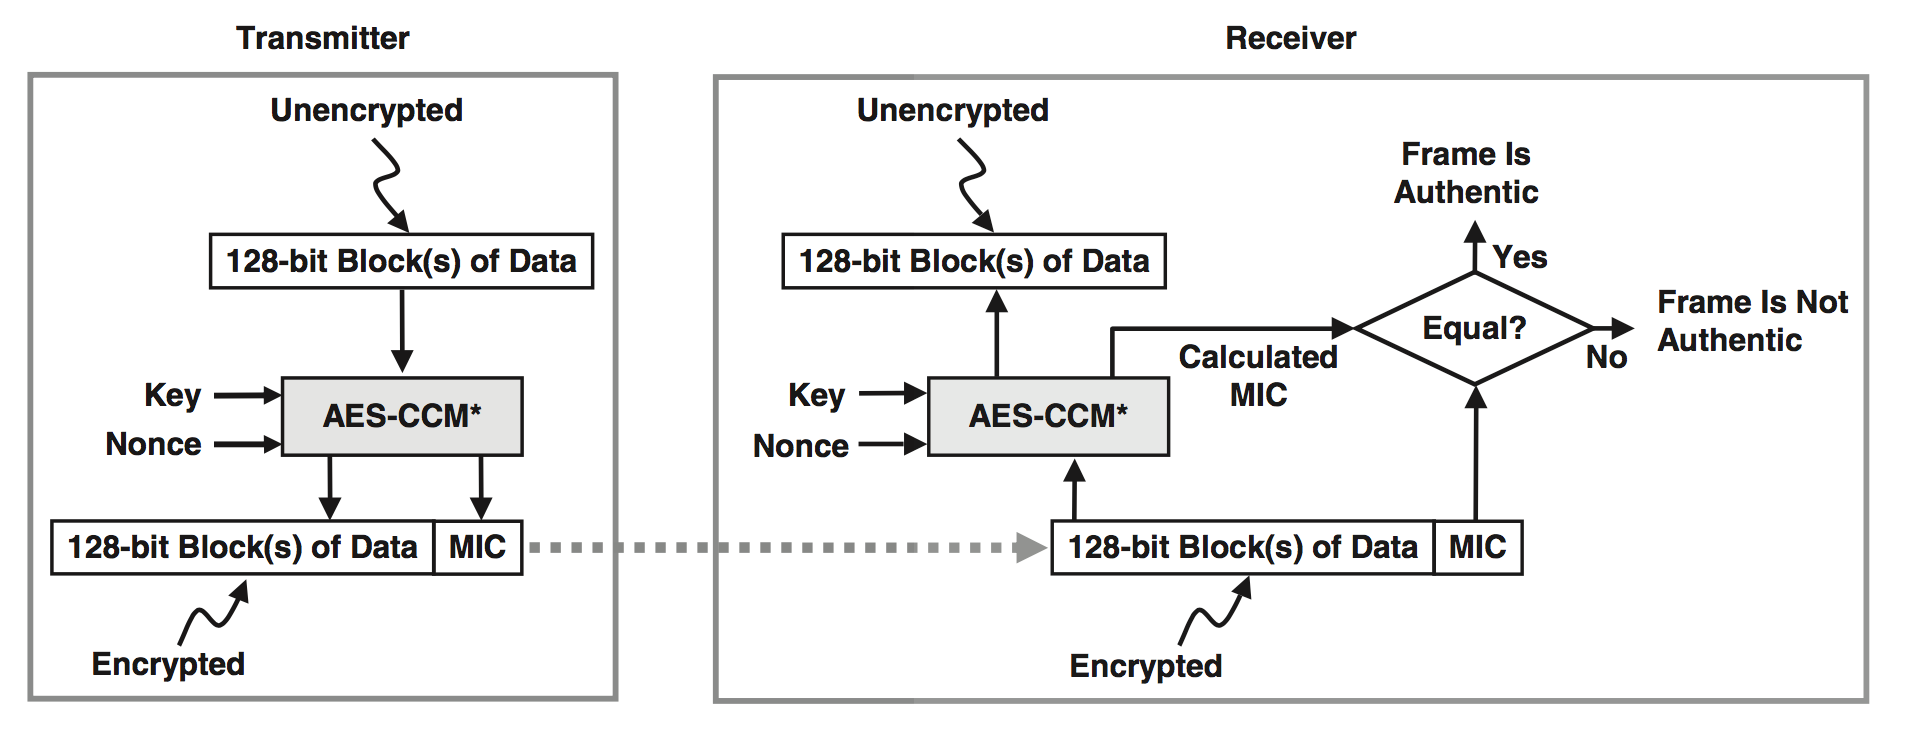
\includegraphics[width=11.5cm,height=12cm,keepaspectratio]{frame_encryption}
\centering
\caption{Frame Encryption}
\end{figure}

The parameter \emph{"nonce"} is a 13-octet string which both the transmitter and the receiver can obtain starting from these three fields of auxiliary header: \emph{security control}, \emph{frame counter} and \emph{source address}.\\
The \emph{MIC} block is nothing but the generated MAC, which can be even called \emph{Message Integrity Code}.

\subsubsection{Replay Attacks Protection}
\bigskip
We have already mentioned that ZigBee offers protection from replay attacks, using a frame counter.\\
More in details, every node in the network has a 32-bit frame counter which is incremented at every packet transmission.\\
Besides, each device tracks the previous frame counter of every node with which it has communicated because, doing this way, if a node receives a packet from another node with the same or lesser frame counter value than it had previously received, the packet will be dropped.\\
It is important to say that the frame counter is reset to 0 when the Trust Center updates the network key.

\subsubsection{Device Authentication}
\bigskip
Clearly, only authorized and authenticated devices can join the network.\\
The Trust Center is responsible to accept new devices that want to join the network, but before doing that the device must be able to receive a network key and set proper attributes within a limited given time to be considered authenticated.\\
More in details, there are two different procedures for authenticating devices:

\begin{itemize}
\setlength{\itemindent}{+4mm}
\item[$\bullet$] \emph{Standard (Residential) mode}: if the new joining device already has a pre-configured network key (unlikely), it will receive an all-zero network key from the trust center as part of the authentication procedure.\\
If the new device does not have a network key and not even a link key (which must be known by the Trust Center obviously), the TC  sends the network key in plain-text, which is a quite important vulnerability.\\
Since the new device does not know the address of the trust center, it will use the source address of the received message to set the trust center address.

\item[$\bullet$] \emph{High Security (Commercial) mode}: in this second, and more secure, mode the Trust Center never sends the network key over an unprotected channel.\\
If the device has a valid pre-configured link key, global or unique, to communicate with the TC, then this last one will send the network key to it, and will consider it as authenticated.\\
A global link key requires less memory to the Trust Center, but it is less secure than the unique link key.\\
Instead, if no pre-configured link key is owned by the device, then the Trust Center expects it to have, at least, the master key by which it is possible to start the key establishment protocol, after that the device and the TC will share the link key.\\
The new device has a limited time to complete the key establishment, otherwise it has to leave the network and retry the authentication procedure again.\\
When and if the link key is confirmed, the Trust Center considers the device as authenticated for commercial mode, and can send the network key to it through a secure channel thanks to the just established link key.\\

This second mode seems to be more secure than the previous one, and surely it is, but actually it has a vulnerability: if the new device does not share a master key with the Trust Center, this last one will send it over an unprotected link. 

\end{itemize}

\subsubsection{Network Interference Protection}
\bigskip
It might happen that nearby wireless networks, even Wi-Fi or other ones, create physical interferences to our ZigBee network.\\
Without entering in too many details, it is important to know that ZigBee and IEEE 802.15.4 try to reduce the presence of interferences using low RF transmission power, low duty cycle and the CSMA/CA mechanism.\\
Often, this is not enough, so ZigBee provides two other strategies to avoid interferences:

\begin{itemize}
\setlength{\itemindent}{+4mm}
\item[$\bullet$] \emph{Collaborative}: ZigBee network and other networks work together; in simple words, when one network is active, the other one remains inactive in order to avoid packet collisions.\\
Clearly, this method expects the two networks to share a communication channel to manage the collaboration.

\item[$\bullet$] \emph{Non-Collaborative}: in this second method, ZigBee network has no communication channel shared with nearby wireless networks, but it uses several interferences detection techniques to avoid as many interferences as possible.\\
We will not discuss the following techniques, since they are outside the context, but for completeness I will provide a list of some of them:

\begin{itemize}
\setlength{\itemindent}{+4mm}
\item \emph{CSMA/CA}
\item \emph{Signal spreading-spreading methods}
\item \emph{Frequency Channel selection}
\item \emph{Adaptive Packet Length Selection}\\
\end{itemize}

\end{itemize}


We conclude this section saying that ZigBee takes care about security, as we have understood so far discussing its security measures.\\
But we have also seen some important vulnerabilities in the exchange of keys, that, just right now, makes the protocol not perfect at all.\\
This is not surprising since ZigBee was designed to keep devices low-cost and low-energy.
In the next section we are going to discuss the most relevant ZigBee vulnerabilities.


\clearpage
\section{ZigBee vulnerabilities}
\bigskip
The aim of this section is to discuss the most relevant ZigBee vulnerabilities and some practical attacks, and related tools, to exploit a ZigBee network.\\
Some of them are related to the specific implementation, while some others are strictly related to the protocol itself.\\
Let's see each of them in details:

\begin{itemize}
\setlength{\itemindent}{+4mm}
\item[$\bullet$] \emph{Key storage}: previously, we mentioned that ZigBee assumes that keys are stored securely within the devices, but this is not always respected.\\
If an attacker is able to extract the network key from a network device, then all the communications within the network will be at risk.

\item[$\bullet$] \emph{Key transportation}: we have seen before that if the Trust Center operates in standard (residential) mode, it could happen that the network key is sent in plain-text; clearly, this is a quite important vulnerability since we transmit the key shared by all the devices within the network to send broadcast messages with no protection at all, compromising the whole network.

\item[$\bullet$] \emph{Ghost Attack}: frame counter checks allow recipient devices to ignore duplicate messages, but a \emph{Denial Of Service (DOS)} vulnerability persists: if an attacker crafts an authentic message and replay it, the recipient will discard it but it will spend time and energy to check its validity.\\
Said that, if an attacker performs tons of replay attacks against the same target, the battery life of this last one will be drastically reduced (especially considering that we are talking about low-power devices).

\item[$\bullet$] \emph{Predictable sensor polling rates}: as we know, end devices can put themselves in sleep mode and wake up at regular intervals to poll the coordinator for data inputs or, in non-beacon mode, when it receives a beacon from the coordinator, in order to save their battery-life.\\
This mechanism gives the attacker an advantage: it can send crafted messages to the device at regular intervals even if it is not necessary, forcing it to wake up and process the received messages.\\
Switching from sleep mode to active mode requires a quite big amount of energy, as well as processing invalid messages, as we have just seen.\\
So, this is nothing but an extension of the previous Ghost Attack, which has been proved to be extremely effective.

\item[$\bullet$] \emph{Manufacturer-defined Link Keys}: manufacturers set default link keys within their devices, and these keys are used by them to join ZigBee networks when the device is unknown to the TC and has no specific authorization associated to it.\\
This is a very bad choice, in fact this means that an attacker can join the network using a device with no pre-established authorization but from a trusted manufacturer, then collect several information about the network it is going to hack in the future.

\item[$\bullet$] \emph{Association Flooding}: by default, there is no integrity checks on acknowledgment packets, therefore an attacker is able to send fake ACK to devices, and they will be considered as authentic.\\
An attacker, within an already compromised network, can keep on reading messages sent by a device even if the respective recipient is not responding, simply sending fake ACK packets to the sender every time it sniff a message from it. 

\item[$\bullet$] \emph{No protection from DOS attacks}: ZigBee has no known denial of service protection mechanisms.\\
There are several ways to perform a DOS attack against a device:


\begin{itemize}
\setlength{\itemindent}{+4mm}
\item \emph{Set the frame counter to its maximum value}: an attacker can send a frame to the victim device setting the frame counter field to the largest acceptable value.\\
Doing this, all the messages that will be sent to the victim device after this one will be rejected since they have a frame counter value smaller than the one received by the attacker.\\
This is the simplest DOS attack, but fortunately it is possible only in those situations where there is no integrity check on the frame, hence when we do not exploit the AES-CCM* mechanism seen before.\\

\item \emph{Flooding}: it consists in the simple sending of tons of messages towards victim devices. For instance, an attacker could replay all the messages it is able to craft (or create legit messages, if it already knows the network key).\\
This kind of attack where the replay messages are sent to all the network devices is called \emph{broadcast storm attack}.\\

\item \emph{Physical Jamming}: this is a physical attack which involves tools able to cause signal interferences big enough to prevent communication among devices.\\

\item \emph{Sinkhole attack}: this attack consists in sending messages in the network in order to compromise communication, altering the routing tables and redirecting the traffic to a fake device through fake routing paths, which cannot be able to carry on the transmission.
\end{itemize}

\item[$\bullet$] \emph{No key re-using control}: a device is allowed to join the network using the same link key several times (even forever if no explicit constraint is specified), but this is a poor choice because if an attacker is good enough to steal the link key of the device, then it will be able to spoof the authentic device credentials and join the network pretending to be it.

\item[$\bullet$] \emph{Trap networks}: since a ZigBee device connects directly to the first available network (or probably the one ) without asking anything to the user, then an attacker could create a fake network which would work as a kind of trap for the device.

\item[$\bullet$] \emph{Statistical attacks}: 



\end{itemize}

















\end{document}



































